\documentclass{article}
\usepackage{graphicx} % Required for inserting images
% \usepackage{biblatex}
% \addbibresource{bibliography.bib}
\usepackage{natbib}
\usepackage{multibib}
\newcites{spec}{Project Specification References} % Creates a new citation command \citespecspec
\bibliographystyle{unsrt}
\bibliographystylespec{unsrt}
\usepackage{wrapfig}
\usepackage{subfigure}
\usepackage{verbatim}
\usepackage{tikz}
\usetikzlibrary{shapes.geometric, shapes.arrows, positioning, fit, backgrounds, arrows.meta, calc}
\usepackage{float}
\usepackage{url}
\usepackage{listings}
\usepackage{xcolor}
\lstdefinestyle{pythonstyle}{
    language=Python,
    basicstyle=\ttfamily\small,
    keywordstyle=\color{blue}\bfseries,
    stringstyle=\color{red},
    commentstyle=\color{gray}\itshape,
    numbers=left,
    numberstyle=\tiny\color{gray},
    stepnumber=1,
    numbersep=8pt,
    frame=single,
    breaklines=true,
    showstringspaces=false,
    captionpos=b
}
% \AtEveryBibitem{%
%   \clearfield{year}%
% }
\usepackage[a4paper, total={7in, 10in}]{geometry}

\title{CS310 Final Report:\\ Application for Identifying Driving Mistakes Using Computer Vision}
\author{Artemiy Brukhno}
\date{April 2026}

\begin{document}

\maketitle

\section*{Abstract}
\begin{comment}
- I've never seen lists in an abstract before. Please investigate whether they are appropriate. To be honest, I don't know whether that list is appropriate in general. Why talk about something which you're not doing?
- In the abstract, you mention "the proposed mobile application" as if you'd already mentioned that you were proposing a mobile application.
- The abstract, in general, is quite descriptive ("we will do X", "we will do Y"). Please refer to the lectures for what an abstract should contain.
\end{comment}
Learning to drive has become a necessary process for the majority of people in the modern world. According to the Driver and Vehicle Standards Agency (DVSA), it takes people "on average 45 hours of driving lessons with a driving instructor plus 22 hours of private practice", and "people who combine their driving lessons with private practice are 50\% more likely to pass the driving test". Driving lessons aim to 
\begin{enumerate}
    \item teach the student \textit{how to drive} the vehicle (pedals, steering etc.), and 
    \item teach them how to \textit{behave} in order to drive \textit{safely} (checking mirrors, assessing hazards on and around the road, etc.).  
\end{enumerate}
In this project we focus on the second goal. \\

It is often difficult to track which behavioural mistakes are most common during driving lessons and to identify patterns and specific areas for improvement from session to session. This is especially true during private practice with family and friends who do not have teaching experience - and may have subjective biases. To this end, the proposed mobile application aims to objectively identify faults and track progress through consecutive driving sessions. The application will use computer vision, including deep learning, to analyse synchronised footage from a cabin-facing camera (e.g. mobile phone front camera) and an external dashcam in order to assess the driver's behaviour corresponding to the vehicle's movement and road environment. After each session, the app will provide feedback on the driver's actions and habits, helping them by identifying mistakes, tracking their progress and guiding improvement. The application will allow users to reduce their tendency to make common mistakes faster, decreasing the number of driving lessons needed for learning to drive safely and passing the test.

\newpage

\section{Introduction}
\begin{comment}
The report should be a self-contained document, so you should provide an introduction to the problem or area the work is addressing. You may wish to include some comments on your motivation for this such as the importance/timeliness of the investigation.

You should include a copy of the original Project Specification as an appendix and can refer to this when appropriate.

Make sure the objectives of your project are clear and clarify why this is a significant undertaking of suitable level for a third year project in your subject.
\end{comment}

Driving remains one of the most dangerous routine activities in the UK. In the UK, around five people are killed and 80 are injured every day due to driving-related incidents \cite{govuk_casualties_2024}. The vast majority of driving accidents occur due to driver error - most often stemming not from a fundamental inability to operate the vehicle, but from behavioural mistakes, namely lack of awareness \cite{road_accident_data, dia_collisions}.\\

Driver Monitoring Systems (DMS) are a technology aimed at tracking driver behaviour using a variety of sensors, including in-cabin video footage. They have recently been designated as an essential safety component in modern vehicles by EU regulation \cite{eurlex_2019_2144}. Most current DMS’ are proprietary - either made by traditional car companies (Toyota \cite{toyota_tmate}, JLR \cite{jlr_dms_news}) or by companies selling hardware/software packages (SmartEye \cite{smarteye_ai}, Nauto \cite{nauto_platform}). While some open-source projects, such as OpenPilot \cite{commaai_openpilot} and ZenRoad \cite{zenroad_app}, also exist, both proprietary and open-source solutions focus on two distinct areas: driver distraction, using in-cabin footage; or the car’s movement, using dash-cam footage. However, no system combines the two sources of data.\\

% Can you show some screenshots of existing tools in the Introduction section?

The central idea for this project is that a truly comprehensive understanding of driver behaviour cannot be determined solely from observing either the driver or the car’s movement in isolation. Instead, our objective is to implement a multi-modal approach, synchronising the driver’s state with the external road environment and the movement of the vehicle. As such, the aim of this project is to create a system capable of identifying driving mistakes, namely failure to check mirrors before manoeuvres, by processing synchronised dash-cam footage and in-cabin footage. The project will leverage computer vision techniques, such as head pose estimation from in-cabin footage to establish driver gaze direction, as well as neural networks or optical flow from dash-cam footage to identify car manoeuvres, such as lane changes and turns.\\

A system capable of objectively identifying driver errors has numerous potential applications, such as:
\begin{itemize}
    \item A feedback tool for learner drivers.
    \item Improving usage-based car insurance analytics.
    \item In-car accident prevention/alert systems.
\end{itemize}

In order to establish a clear goal and evaluation criteria, this project will focus on the learner driver use-case. The minimum viable product (MVP) is a web application for post-hoc analysis, processing synchronised dash-cam and in-cabin footage to identify and timestamp specific driving errors. The application aims to improve the quality of driving sessions with friends and family, who are less likely to spot subtle mistakes like mirror-checks \cite{2nd2nonedrivingschoolLearningDrive}. The system's performance will be evaluated by addressing the research question: `Can the system identify driving errors with greater accuracy than a non-professional supervisor?' To this end, a user study will be conducted to quantitatively compare the application's error-detection performance against that of people who are not formally trained as driving instructors.

\newpage

\section{Background}
\begin{comment}
% Can you look into whether the techniques that you're discussing (e.g. "computer vision", "transformers", "neural networks", etc.) need to have the first letter of each word capitalised? I don't think they do but I am not 100% sure. I think names of things (e.g. "Recursive Video Lane Detection", if that is a proposed approach) needs to have its first letters capitalised, but general categories (e.g. "neural networks") do not. But please check.
\end{comment}

This section reviews the key computer vision techniques used in the project, covering lane detection, temporal tracking, gaze estimation and motion estimation as the four core components of the proposed system.

\subsection{Lane Detection}
Lane detection is a well-researched topic within computer vision (CV). It is an essential tool for many modern vehicle features, from lane assist to full self-driving systems. Lane detection aims to detect lane lines or lane areas by either camera or lidar \cite{tang_review_2021}. This project focuses on camera-based perception, due to the cost and scope constraints of using lidar. Classical lane detection methods involved image processing techniques such as Sobel \cite{sobel_1968} and Canny \cite{canny_1986} filters, followed by Hough transform \cite{duda_1972} and curve fitting. However, these methods suffered from poor performance and consistency in varying lighting conditions and faded or obscured lane lines \cite{hillel_2014}. Since the project aims to work on urban roads in different lighting and weather conditions, these methods are not suitable. \\

The modern development of lane detection systems focuses on deep learning to create more robust and adaptable models, specifically using Convolutional Neural Networks (CNNs). CNNs are an advancement of traditional Neural Networks (NNs), with Convolutional and Pooling layers added to the beginning of the architecture \cite{lecun_1998}, generalising NNs to work on images (Figure \ref{fig:cnn_vis}). These layers use convolutions \cite{goodfellow_2016} to extract relevant features from the input, which are then flattened and passed to traditional, fully connected layers for classification. \\

\begin{figure}[H]
    \centering
    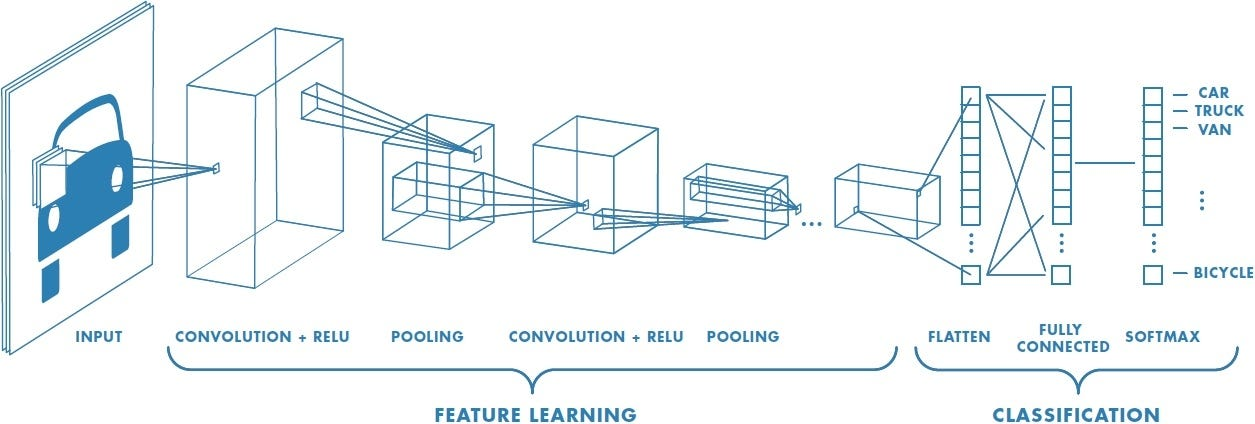
\includegraphics[width=1\linewidth]{research_images/cnn_explanation.png}
    \caption{Visualisation of CNN architecture. Source: \cite{mathworks_cnn}.}
    \label{fig:cnn_vis}
\end{figure}

Existing deep learning-based lane detection methods can be grouped into two categories: two-step and one-step methods \cite{tang_review_2021}. Two-step methods first perform feature extraction using heuristic recognition-based methods and deep learning, followed by post-processing with clustering and fitting. An example of this is LaneNet \cite{wang_lanenet_2018}, which generates a binary segmentation map and per-pixel embeddings, requiring a subsequent clustering step to distinguish individual lane instances. On the other hand, one-step methods can get the detection and clustering results directly from the image. Inspired by single-stage object detectors such as YOLO \cite{redmon_you_2016}, architectures like PolyLaneNet \cite{tabelini_polylanenet_2020} obtain lane curve parameters directly, bypassing the need for heuristic post-processing.\\

Table \ref{tab:lane_model_comparison} details the performance results of several state-of-the-art models on the two primary benchmarks: TuSimple \cite{TuSimple2017} and CULane \cite{CULane2018}. The data for TuSimple is limited to US highways and intersections, while CULane features a range of environments, including urban streets and rural roads, and was collected under more challenging weather conditions such as rain and fog. For this reason, the CULane benchmark is the more relevant one to our project. 

% would be good to show some of the data from TuSimple and/or CULane, especially since you're highlighting special characteristics of the data (weather conditions).

\begin{table}[H]
    \centering
    \begin{tabular}{l l l c c}
    \hline
    \textbf{Model} & \textbf{Backbone} & \textbf{Architecture} & \textbf{TuSimple (Acc \%)} & \textbf{CULane (F1 \%)} \\
    \hline
    SCNN~\cite{pan2018spatial} & VGG-16 & Two-step & 96.53 & 71.60 \\
    LaneNet~\cite{wang_lanenet_2018} & ENet/VGG & Two-step & 96.38 & 51.99 \\
    UFLD~\cite{qin2020ultra} & ResNet-18 & One-step & 95.82 & 68.40 \\
    PolyLaneNet~\cite{tabelini_polylanenet_2020} & EfficientNet-B0 & One-step & 93.36 & 61.79 \\
    LaneATT~\cite{tabelini2021keep} & ResNet-34 & One-step & 95.63 & 76.68 \\
    CondLaneNet~\cite{liu2021condlanenet} & ResNet-101 & One-step & 96.54 & 77.85 \\
    CLRNet~\cite{zheng2022clrnet} & ResNet-101 & One-step & 97.62 & 79.73 \\
    \hline
    \end{tabular}
    
    \caption{Performance comparison of modern lane detection models.}
    \label{tab:lane_model_comparison}
\end{table}


In order to establish if these models would generalise to British streets and consumer hardware (dash-cams), they were also qualitatively tested on the author's self-collected driving dataset (Figure \ref{fig:drive_examples}). The LaneATT model was found to perform the most accurately and reliably. A quantitative benchmark was infeasible for the project, as this would require extensive manual labelling, taking time away from feature development. 

% In Figure 2, it is slightly odd that one of the subfigures relates to "UFLD" before you've mentioned what that is (although I can see that it is represented in Table 1). It'd be good to state what this is.

\begin{figure}[H]
    \centering
    \subfigure[]{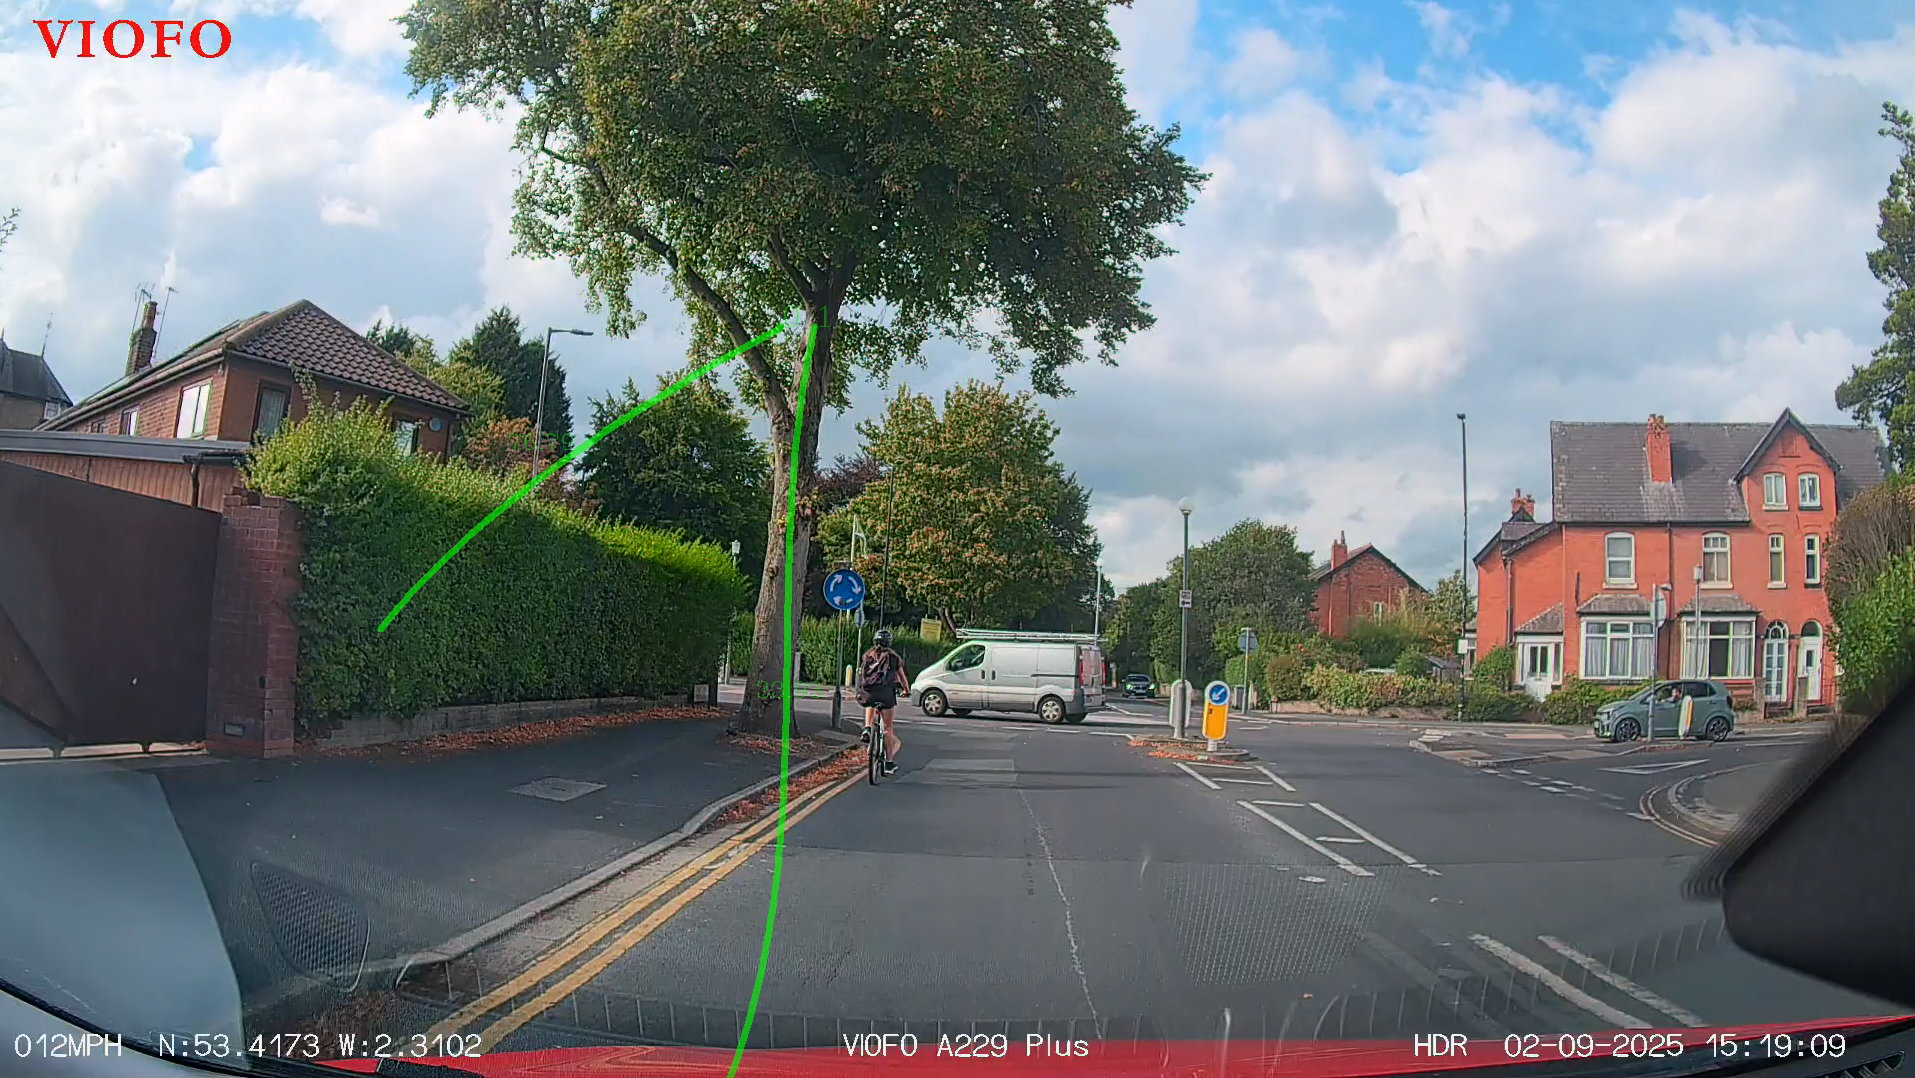
\includegraphics[width=0.329\textwidth]{driving_images/poly_drive.png}}
    \subfigure[]{\includegraphics[width=0.329\textwidth]{driving_images/ufld_drive.png}} 
    \subfigure[]{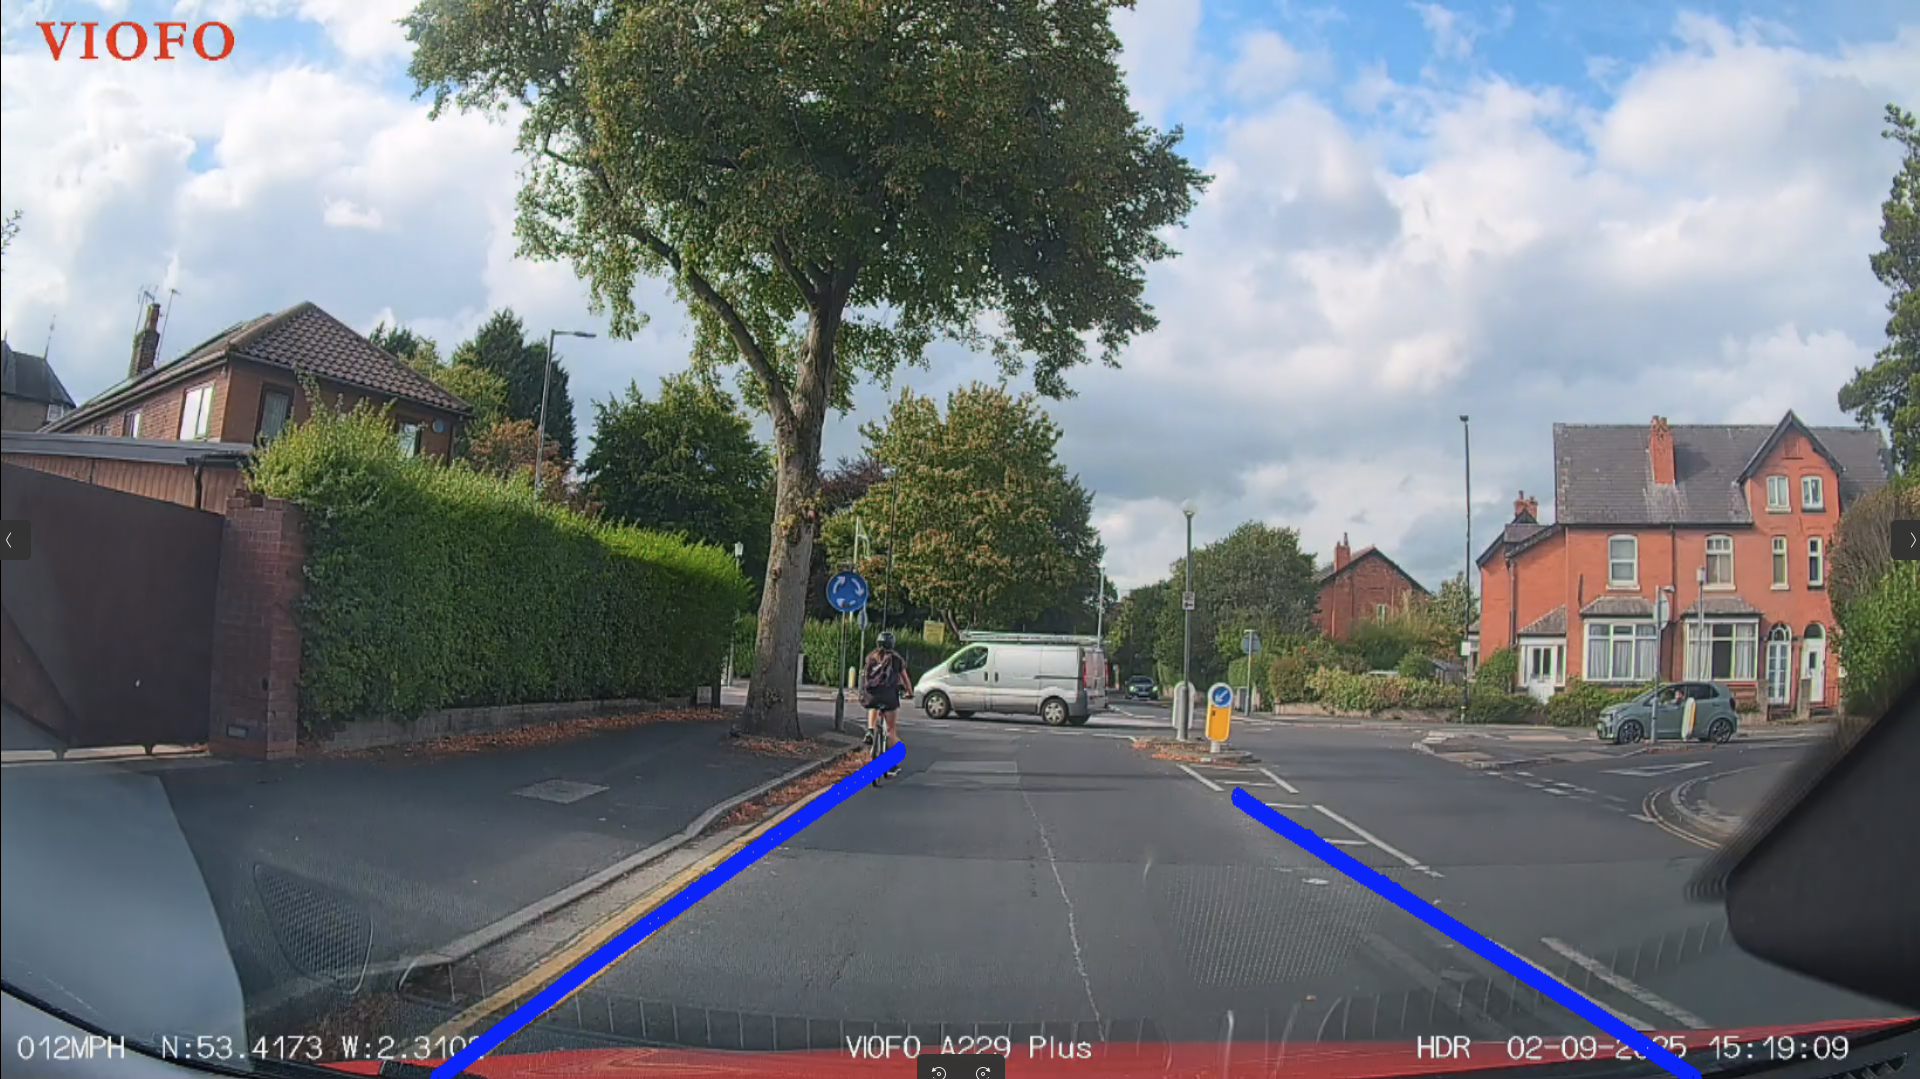
\includegraphics[width=0.329\textwidth]{driving_images/laneatt_drive.png}} 
    \caption{Examples of model performance on a British road: (a) PolyLaneNet. (b) UFLD. (c) LaneATT.}
    \label{fig:drive_examples}
\end{figure}

\subsection{Temporal Tracking}
% "Lane detection is a per-image process, meaning that for each image a new set of lanes is detected. This means that lane information is forgotten on each new frame" - is it? Maybe in the most literal interpretation (one detects lanes in frames and tracks them in videos), but I still think this is a stretch. Consider rewording.
Standard lane detection models process each frame independently, producing a fresh set of detections with no awareness of previous frames. This lack of temporal continuity means that lane identity and position must be re-established every frame, which is insufficient for the project's requirement to track lane changes over time. Lane tracking addresses this by maintaining persistent lane state across frames, predicting the position and movement of lanes in time-series driving data. \\

State-of-the-art research on this subject focuses on directly training NNs, such as Transformers \cite{vaswani2017attention}, with video data as input (rather than images). Models such as RVLD (Recursive Video Lane Detection) \cite{jin_recursive_2023}, which propagates the state of the current frame to subsequent frames, show high-performing results. Another modern approach, used by YOLOP \cite{wu_yolop_2022} and Openpilot \cite{chen_level_2022}, is to train an all-in-one model, which learns lane detection and tracking as well as movement/position estimation, road surface segmentation and object detection all at once. While such methods are currently at the academic frontier, the industry standard remains focused on more classical methods, such as the Kalman Filter. Recent reviews \cite{yurtsever2020survey} confirm that for safety-critical ADAS, separating `perception' (deep learning) from `state estimation' (Kalman filtering) is preferred due to its explainability, whereas the former methods act as a black box once trained. For this reason, the Kalman Filter approach was chosen for the project. \\

The Kalman Filter is a temporal method which works in two phases: prediction and update (Figure \ref{fig:kalman_vis}). The filter stores the last known location and velocity of a lane in a ‘state vector’. It uses the current velocity to predict where the lane should be in the next frame. Next, it observes the actual detection from the model to update this prediction. If a lane is obscured or faded, the filter uses the prediction to `remember' the lane. This makes the system robust to per-frame fluctuations and lighting anomalies, ensuring consistency even when detections are missed.

\begin{figure}[H]
    \centering
    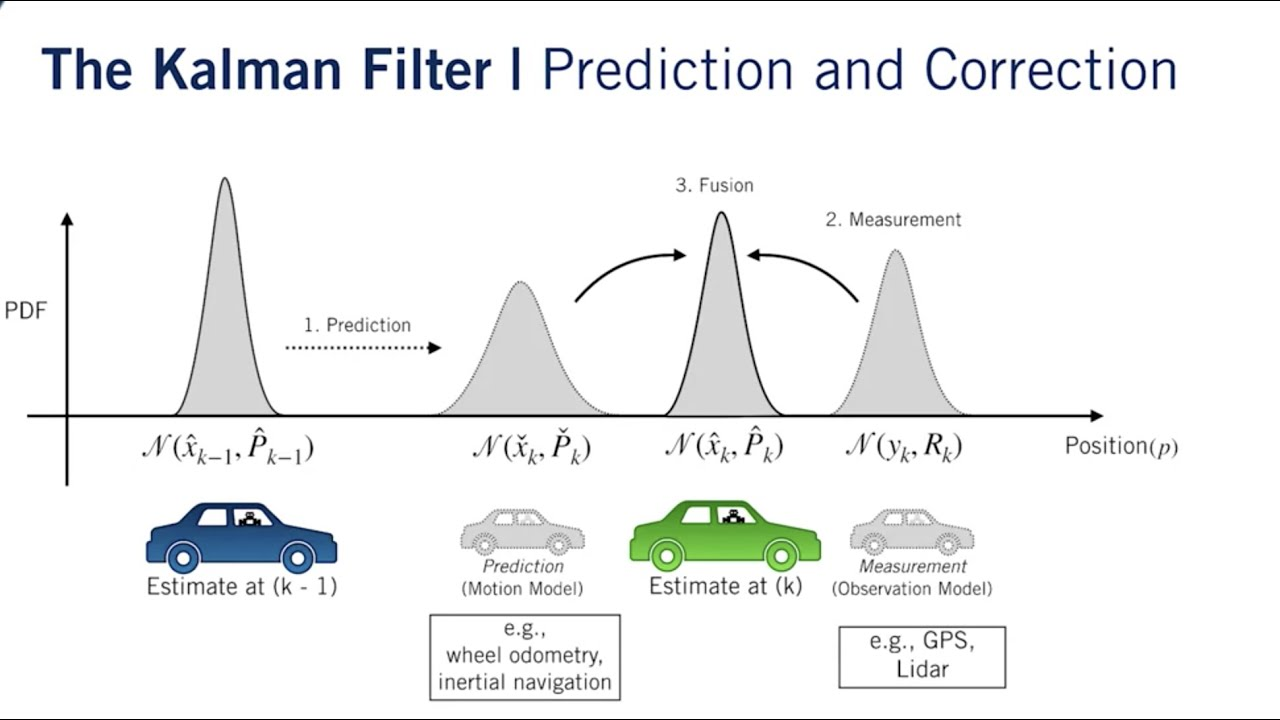
\includegraphics[width=0.75\linewidth]{research_images/kalman_vis.png}
    \caption{Visualisation of Kalman Filter for storing vehicle state. Source: \cite{MachineLearningTV2021Jun}.}
    \label{fig:kalman_vis}
\end{figure}

\subsection{Gaze Estimation}

Gaze estimation is a process used to determine the direction of a person's head. This is achieved through face analysis, which stores the facial orientation and pose. Modern systems, such as Drive Sense \cite{salma_drive_2024}, typically use landmark detectors to extract key points (mouth, eyes, nose) from an image. To establish the angle of the 2D points, the Perspective-n-Point (PnP) algorithm is commonly used. PnP calculates the matrix required to transform a `canonical' 3D face shape to the detected location of the tracked points (Figure \ref{fig:pnpvis}). The matrix consists of the $3\times3$ rotation matrix $R$, followed by a $3\times1$ translation vector $t$, allowing the angles (yaw, pitch, roll) to be calculated.

\begin{figure}[H]
    \centering
    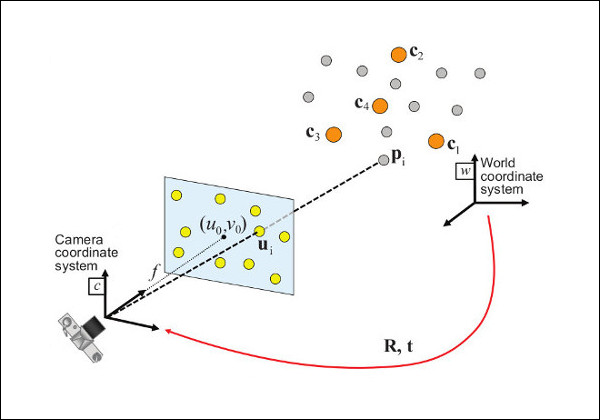
\includegraphics[width=0.5\linewidth]{research_images/pnp.png}
    \caption{Visualisation of the PnP problem. Source: \cite{opencv_pnp}.}
    \label{fig:pnpvis}
\end{figure}

Once angles are extracted, they must be classified into discrete gaze directions (e.g. mirrors or forward). Dimensionality reduction techniques, such as Principal Component Analysis (PCA) \cite{jolliffe2016principal}, are often used to transform the data, for example, from three angles to two, to make clusters of points corresponding to each gaze classification more well-defined.\\

% The final paragraph on page 5 makes lots of claims regarding SVM reliability, safety, consistency, yet provides no evidence:

For the final classification step, a choice exists between unsupervised clustering (e.g. K-Means \cite{macqueen1967some}) and supervised learning (e.g. Support Vector Machines or SVM \cite{cortes1995support}). While K-Means can show the quality of clusters without labels, it often struggles with outliers or classes that occupy narrow areas of the feature space. SVM is preferred for safety-critical applications due to its robustness with small amounts of training data and its explainability. Unlike NNs, which can be a black box, SVMs offer high reliability and consistency, which is desirable when the situation allows for simpler models.

\subsection{Motion Estimation}
\begin{comment}Describe the research conducted into pose/motion estimation techniques, including Visual Odometry and SLAM, and why VO was chosen (we only need local/relative motion, rather than global for our use-case/project and task description). Describe existing solutions and how they work - key-point matching, orb selectors, essential matrix etc. 

FOR TESTING/EVALUATION
Create some sort of ground truth benchmark - using GPS from car??
Then compare results from VO model with/without various features to show addition helps.
\end{comment}

Motion estimation is an essential topic within robotics and autonomous vehicle research, with the aim of identifying the relative direction, speed and position of a camera as it moves through an environment. For this project, motion estimation is used to detect left and right turns (FR3.1.1). Two relevant methods for this are Visual Odometry (VO) and Visual Simultaneous Localisation and Mapping (vSLAM) \cite{taketomi2017visual}. vSLAM constructs a persistent map of the environment (Figure \ref{fig:vslam_example}), and can identify loop-closures to correct for drift accumulation. However, it is considerably more computationally expensive than VO and provides more environmental information than is necessary for this project. Since only local, relative motion is needed for turn detection, VO was selected as sufficient without the overhead of full environment mapping. \\

\begin{figure}[H]
    \centering
    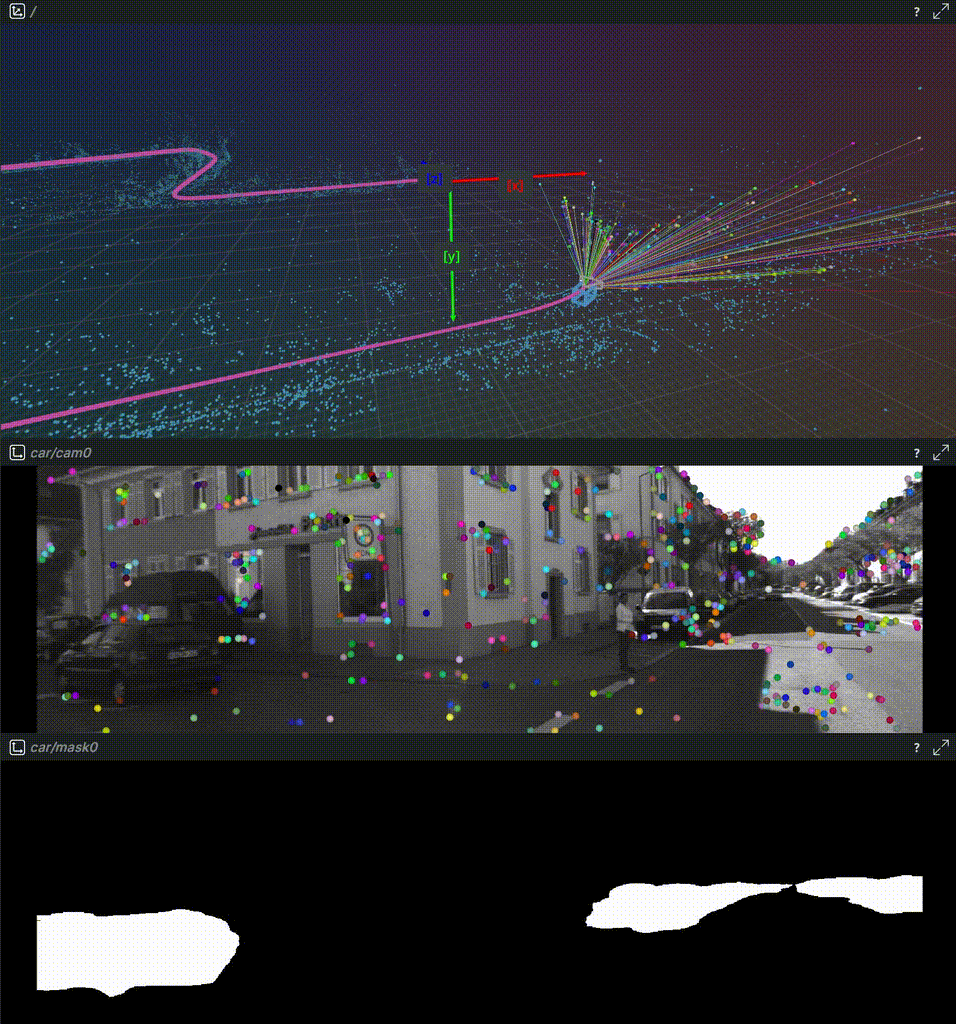
\includegraphics[width=0.75\linewidth]{research_images/pycuvslam_example.png}
    \caption{vSLAM example with vehicle segmentation on the KITTI Stereo Odometry dataset. Source: PyCuVLSAM \cite{korovko2025cuvslamcudaacceleratedvisual}}
    \label{fig:vslam_example}
\end{figure}

VO analyses sequential camera frames to estimate the camera's local motion incrementally. The process begins with keypoint detection, where algorithms such as Shi-Tomasi \cite{shi1994good} or ORB \cite{rublee2011orb} identify distinctive features in each frame. These keypoints are then tracked across consecutive frames using sparse Optical Flow, a technique that estimates the displacement of individual feature points between frames rather than computing motion for every pixel. The Lucas-Kanade method \cite{lucas1981iterative} is commonly used for this, as it is efficient and well-suited to tracking a sparse set of points. For this project, Shi-Tomasi was selected for keypoint detection, as it produces corners with strong gradients in two directions, which is exactly what Lucas-Kanade is designed to track. Alternatives such as FAST or ORB were considered, but these produce lower-quality corners or include binary descriptor computation that is unnecessary when using optical flow for matching rather than descriptor comparison. \\

\begin{figure}[H]
    \centering
    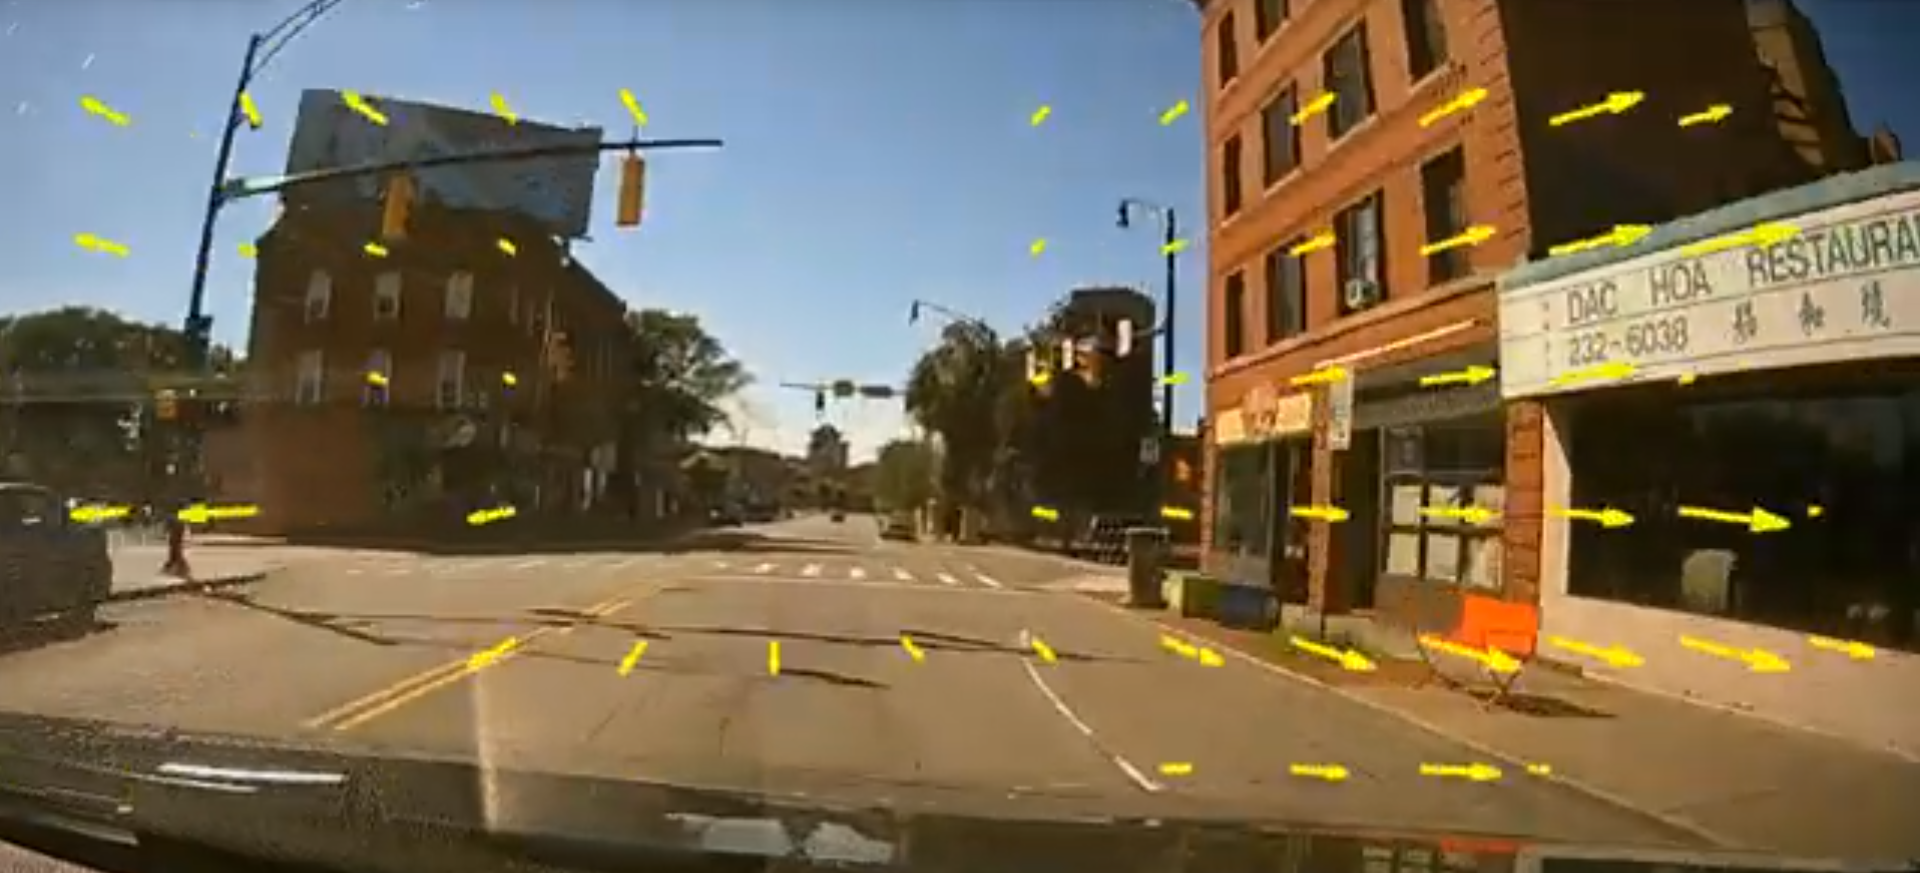
\includegraphics[width=0.75\linewidth]{research_images/optical_flow_ex.png}
    \caption{Optical flow example. Source: \cite{mathworks_optical_flow}}
    \label{fig:optical_flow_ex}
\end{figure}

Once correspondences between keypoints are established, the Essential Matrix is computed from the matched point pairs. The Essential Matrix encodes the geometric relationship between two camera views, and can be decomposed into a rotation matrix $R$ and translation vector $t$ that describe how the camera has moved between frames. This is analogous to the PnP decomposition used in gaze estimation (Section 2.3), but operates on frame-to-frame correspondences rather than a canonical 3D model. Since this project is limited to a single dash-cam, the variant of VO used is monocular, which naturally faces scale ambiguity, meaning it can only obtain relative motion estimates, and the motion estimate is likely to drift over time. \\

One approach for classifying manoeuvres from VO output, introduced by Zekany et al. \cite{zekany2022finding}, involves using a deep learning VO model to estimate the ego-vehicle trajectory and comparing a sliding window of this trajectory against a predefined library of reference manoeuvres using Dynamic Time Warping (DTW), a classical distance metric for time-series comparison. However, the use of a deep learning model for the VO step makes the trajectory estimation itself a black box. As noted in recent reviews \cite{yurtsever2020survey}, separating perception from state estimation is preferred in safety-critical applications due to its explainability, and simpler rule-based methods are favoured where the task allows for it. Since this project requires only binary left/right turn detection rather than classification of a broad range of complex manoeuvres, a threshold-based approach to yaw accumulation is adopted instead, where each detection decision can be directly traced to interpretable thresholds.

\subsection{Background summary}
\begin{comment}
I think it'd be good to have a summary subsection at the end of Section 2, making it clear which parts of Section 2 are going to be used in your work.
\end{comment}

\newpage

\section{Design and Development}
\begin{comment}
Provide an overview of your work so far. This should include:

    - Technical Content - what work have you done? You should provide a meaningful discussion of the significant aspects rather than simply saying "I did x, y and z". This is necessary to show you've actually done it and in order for your assessor to award marks according to the assessment criteria.
    - Progress - review your progress against the original timetable. If unexpected problems or delays have occurred, how have you dealt with the problem?
\end{comment}

% ...
The project was implemented using a modular architecture, separating code into distinct sub-modules (Figure \ref{fig:folders}), corresponding to the Must-Have objectives: Lane Detection/Tracking (FR1.2/3), Gaze Estimation (FR1.4) and Web Application (FR2). This left room to extend the project with features, specifically those detailed in the Should-Have requirements, and to improve individual features further without affecting the rest of the system. Features added on top of the Must-Have requirements were FR3.1 and FR4.1, since these were decided to have the largest impact for the project with the time remaining. While the modular approach did add some complexity with an additional necessary module to compile the outputs into the final analysis (`combined analysis’), the benefits to maintainability and extendibility were decided to outweigh this.\\

The \texttt{combined\_analysis} module runs each module separately, and aggregates the results from each in order to assess the safety of manoeuvres. It does this by maintaining a \texttt{Safety Monitor} class, storing an event buffer which is cross-referenced when a manoeuvre is detected, determining the safety classification that is given.

\begin{figure}[H]
    \centering
    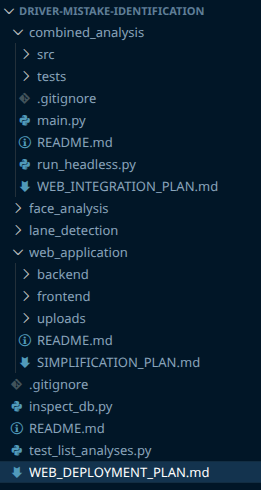
\includegraphics[width=0.3\linewidth]{project_management_images/folder_structure.png}
    \caption{Folder structure showcasing the modular structure of the project.}
    \label{fig:folders}
\end{figure}

\subsection{Resources and Tools}
Rather than training models from scratch, the project utilises pre-trained models and standard tools to perform the analysis. Python, thanks to its robust ecosystem of data processing libraries, is the language chosen for most state-of-the-art ML research, so we use it in this project. While there are two prominent Python libraries for ML and NN development, PyTorch \cite{paszke2019pytorch} and TensorFlow \cite{abadi2016tensorflow}, we are only able to use models implemented in the PyTorch library. This is because it was discovered that the available development GPU (RTX 5070Ti) operates using a new CUDA compatibility protocol, `Compute Capability 12.0’, which is not yet supported by TensorFlow.\\

\subsection{Lane Change Detection (FR1.2 \& FR1.3)}
Lane detection allows us to represent the position of the car relative to the road, which in turn informs us of the vehicle’s movement, and specifically any manoeuvres that it performs. While the model we chose to use in the end was LaneATT, the process to come to this conclusion came with several challenges.\\

One problem was that the datasets that are used for training models (TuSimple, CULane) contain only straight or slightly curved road examples. Because of this, roundabouts and roads with significant curvature fail to be detected. Additionally, there do not exist any specific datasets or research papers that investigate the specific case of driving on roundabouts. As such, roundabouts remain a limitation of the project.\\

Another limitation identified was the generalisability of many models to consumer dash-cam hardware, with several models showing poor performance on the self-collected dataset (Figure \ref{fig:drive_examples}). A possible explanation is over-fitting to the camera parameters used during dataset collection. When tested on footage from cameras with different fields of view, warped lenses or compression artefacts, detection accuracy degraded significantly. The attention mechanism used by the LaneATT model may explain its increased robustness under these conditions, although this topic is not discussed in the literature.\\

Lane tracking was implemented by storing lane information in `LaneTrack’ objects, which use a Kalman filter to store and update their state. An overall `LaneTracker’ object is responsible for matching previously stored lanes to newly detected lanes. Initially, the Hungarian algorithm \cite{kuhn1955hungarian} was used for this matching process, however it always produces a complete matching even when distances between lanes are very large. This resulted in scenarios where the system matched lanes across the entire image, if a lane on the left side of the image stopped being tracked, but a new lane was detected on the right side. \\

Instead, we switched to a ‘closest first’ approach with a gate-based cut-off (Listing \ref{lst:lane-tracker-gated}). The first-closest pairs are matched to each other, and if a pair’s distance exceeds the cut-off point, they are not matched and the detected lane is stored as a new lane rather than updating an existing one, while the stored lane is counted as a miss. This change eliminated such scenarios and made the tracking work more reliably in practice (Figure \ref{fig:cars_lanes}).\\

\begin{lstlisting}[
    style=pythonstyle,
    caption={Closest-first gated data association for lane tracking (key logic)},
    label={lst:lane-tracker-gated}
]
class LaneTracker:
    def update(self, detections):
        # Predict existing tracks
        predictions = [t.predict() for t in self.tracks]

        # If no detections: count misses, prune stale tracks, then check lane-cross events
        if not detections:
            self._prune_tracks()
            self.cross_events = [
                {"track_id": t.id, "direction": d}
                for t in self.tracks
                if (d := t.check_lane_cross())
            ]
            return

        # Distance-based cost between predicted and detected lane polynomials
        C = self._calculate_cost_matrix(predictions, detections)

        # Closest-first matching with gating
        matches = []
        Cg = C.copy()
        while Cg.size > 0:
            r, c = np.unravel_index(np.argmin(Cg), Cg.shape)
            if C[r, c] > 300:  # gate threshold
                break
            matches.append((r, c))
            Cg[r, :] = np.inf
            Cg[:, c] = np.inf

        matched = set()
        for r, c in matches:
            self.tracks[r].update(detections[c])
            matched.add(c)

        # Unmatched detections initialise new tracks; unmatched tracks accumulate misses
        self._create_new_tracks([detections[i] for i in range(len(detections)) if i not in matched])
        self._prune_tracks()
\end{lstlisting}


\begin{figure}[H]
    \centering
    \subfigure[]{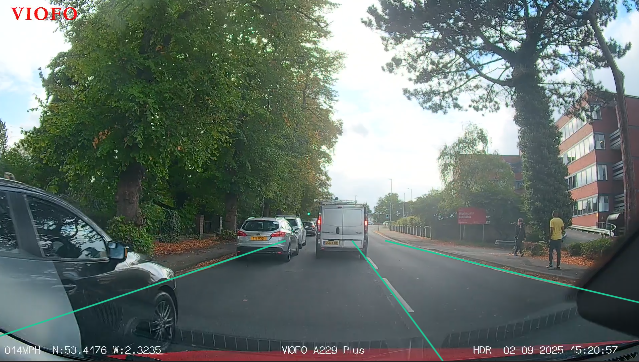
\includegraphics[width=0.45\textwidth]{driving_images/car_obstruction_marsland.png}}
    \subfigure[]{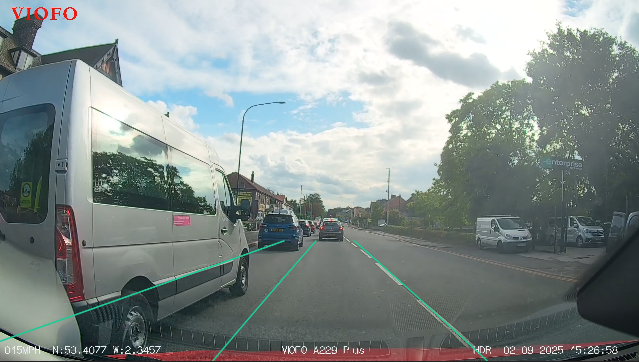
\includegraphics[width=0.45\textwidth]{driving_images/car_obstruction_2.png}} 
    \caption{Example frames of cars obstructing lane, with lane remaining tracked.}
    \label{fig:cars_lanes}
\end{figure}

The lane tracker stores the position of each lane relative to the image centre. Lane change detection is performed by checking whether a tracked lane crosses the centre of the frame, with lane velocity used to determine direction and reduce false positives caused by old or faded lane markings. Detected lane change events are stored in the \texttt{Safety Monitor} class' buffer.

\subsection{Turn Detection (FR3.1.1)}
Turn detection is necessary to extend mistake identification beyond lane changes to include failures to check mirrors before turning at junctions, a common fault on driving tests. Since the project does not have access to vehicle telemetry (steering angle, GPS waypoints), the only available signal is the road-facing video itself. This motivated the use of Visual Odometry (VO) to estimate the vehicle's heading change over time.\\

Several established open-source VO and Visual SLAM systems were evaluated. DROID-SLAM \cite{teed2021droid} produced high-quality reconstructions on benchmark datasets but required a specific CUDA toolkit version incompatible with the project's CUDA 12.0 environment, and its dense bundle adjustment was prohibitively slow for the project needs even while running on the DCS batch compute systems. TartanVO \cite{wang2021tartanvo}, a learning-based approach, generalised poorly to dash-cam footage, likely because its training data (TartanAir) consists of synthetic indoor and outdoor scenes with very different visual characteristics to UK road footage. DeepV2D \cite{teed_deepv2d_2020} suffered from similar dependency conflicts and, like the others, operated as a monolithic system whose internal parameters were difficult to tune for the specific failure modes observed (e.g.\ drift during stops at traffic lights, erratic estimates when large vehicles fill the frame).\\

Because the project only requires yaw-based turn detection rather than metrically accurate 3D reconstruction, a custom lightweight VO pipeline was developed instead. This offered full control over each processing stage, making it straightforward to diagnose and fix failure modes as they arose, an advantage that proved critical during iterative development. Existing functions provided by the OpenCV Python library made creating this pipeline straightforward to implement. The pipeline operates by extracting and matching visual features between consecutive frames, then estimating the relative camera motion from the resulting point correspondences. \\

Frame-by-frame, we perform a centre crop (75\%) of the road video. The crop removes the image periphery where radial lens distortion is strongest, avoiding the need for a full undistortion step that would add latency and introduce interpolation artefacts. This also removes external, static elements such as the hood of the car or stickers on the windscreen. For each frame, a Mask R-CNN \cite{he2017mask} (ResNet-50 FPN V2) instance segmentation model identifies dynamic objects (cars, pedestrians, cyclists, buses and trucks) and produces a binary mask. This masking step is essential because optical flow from moving vehicles would otherwise be interpreted as camera ego-motion, causing large errors in the estimated rotation. Early iterations without dynamic masking produced frequent false turn detections when vehicles overtook or braked ahead, as the dominant flow from these objects overwhelmed the static background signal.\\

% TODO: Insert images of tracking results with and without the masking

Features are detected only on the unmasked (static) regions using a grid-based bucketing strategy, which divides the image into a $4 \times 6$ grid and runs \texttt{goodFeaturesToTrack} independently in each cell. Without bucketing, detected features would be evenly spread out through the image, with many points detected in non-feature-rich areas of the image, such as repeating textures on housing tiles and roads (Figure \ref{fig:points_houses}). This meant that in subsequent frames where points were detected close to here, they would be matched to each other despite not actually corresponding to the same point. This essentially caused a high degree of noise within the tracking algorithm due to non-identifiable point-matching. This was fine while the car was moving, but when it was stationary or moving very slowly, the noise took over the tracking and caused extremely sharp, inaccurate pose predictions.\\

\begin{figure}[H]
    \centering
    \subfigure[]{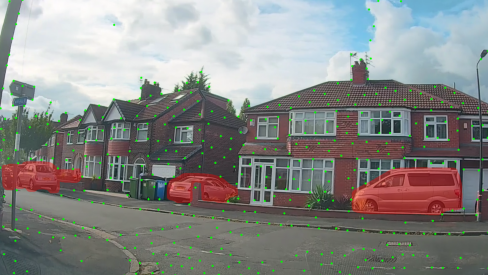
\includegraphics[width=0.45\textwidth]{driving_images/house_without_grid.png}}
    \subfigure[]{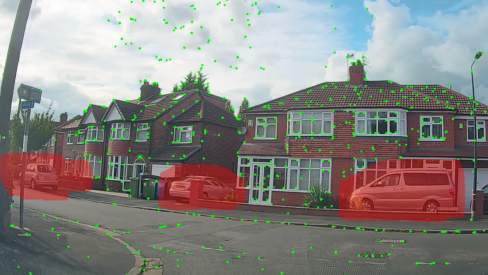
\includegraphics[width=0.45\textwidth]{driving_images/houses_with_grid.png}} 
    \caption{(a) Tracked features without bucketing: points are evenly spread out on road and brick textures. (b) Tracked features with bucketing: Points cluster to feature-dense areas of the image.}
    \label{fig:points_houses}
\end{figure}

Features are tracked between consecutive frames using Lucas-Kanade optical flow. A forward-backward consistency check \cite{kalal2010forward} is applied. This means that points are tracked forward to the current frame, then backward to the previous frame, and only matches with a re-projection error below 0.5 pixels are retained. This eliminates poorly tracked points that would otherwise introduce noise into the pose estimate, particularly near the edges of the dynamic object mask, where partial occlusions by cars and people caused errors in tracking. The essential matrix is then estimated via RANSAC \cite{fischler1981random}, and the relative rotation and translation are recovered using \texttt{cv2.recoverPose}. One major improvement was to reject pose estimations between frames which are deemed physically implausible. A common example was if the calculated rotation exceeded an unrealistic threshold ($\sim$28\textdegree\ ), which often occurred during slow-moving sequences due to unexpected sources of noise.\\

Raw pose estimates are accumulated and fused through a 12-state Kalman filter tracking position ($x, y, z$), orientation (roll, pitch, yaw) and their velocities. The Kalman filter serves two purposes: it smooths the noisy frame-to-frame VO estimates into a coherent trajectory, and it maintains a reasonable state estimate during periods where VO measurements are unreliable. To achieve the latter, the measurement noise covariance is adjusted dynamically based on tracking confidence. When the vehicle is moving and tracking is successful, standard noise is applied. When the vehicle is stationary (low optical flow), higher confidence is placed on the prediction to prevent drift from noisy near-zero estimates. When the segmentation mask covers most of the frame (a ``blind'' condition occurring in heavy traffic), the filter almost entirely trusts its own prediction, as there are insufficient static features to produce a meaningful VO measurement.\\

\begin{figure}[H]
    \centering
    \subfigure[]{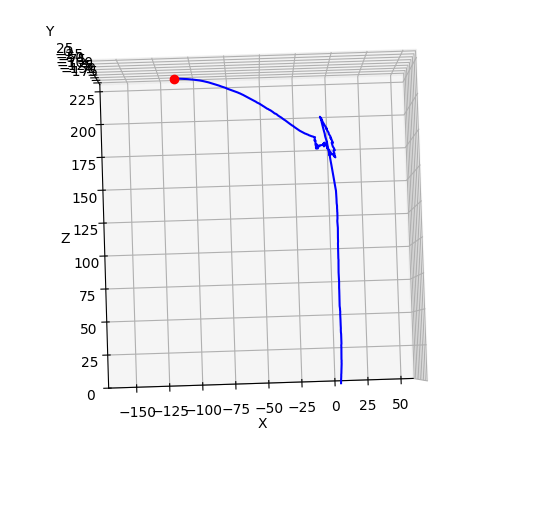
\includegraphics[width=0.45\textwidth]{driving_images/tracking_without_kalman.png}}
    \subfigure[]{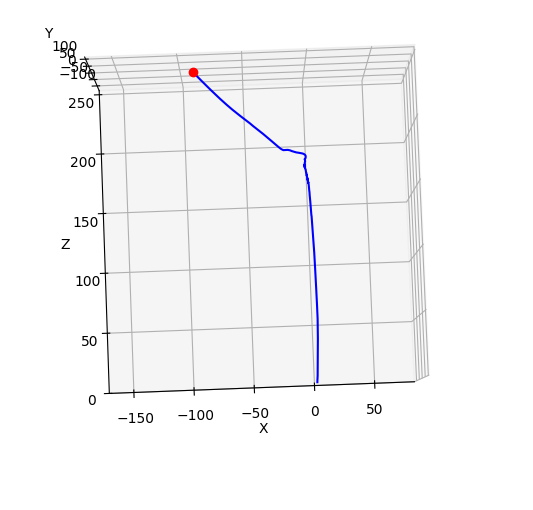
\includegraphics[width=0.45\textwidth]{driving_images/tracking_with_kalman.png}} 
    \caption{(a) Tracking example with no Kalman filter or implausible-frame rejection. (b) Tracking example with Kalman filter and frame rejection.}
    \label{fig:kalman_comparison}
\end{figure}

Turn detection monitors the accumulated yaw rotation via the \texttt{TurnDetector} class. An early approach decomposed Euler angles from the accumulated rotation matrix, but this produced sign flips in long videos where the total rotation grew large, causing left turns to be misclassified as right turns and vice versa. Instead, yaw is now integrated directly from each frame's small relative rotation, where the Euler decomposition is always well-conditioned. A turn event is triggered under one of three conditions: (1) the accumulated yaw exceeds 30\textdegree\ and at least one frame exhibited sharp rotation ($>$0.6\textdegree/frame), distinguishing genuine intersection turns from gradual road curvature; (2) the accumulated yaw exceeds 80\textdegree\ regardless of sharpness, to capture long sweeping turns such as roundabout exits; or (3) the accumulated yaw exceeds 15\textdegree\ combined with a sudden spike ($>$8\textdegree\ in a single frame), catching aggressive manoeuvres. A straightness reset clears the accumulator if rotation remains below 0.1\textdegree/frame for 30 consecutive frames ($\sim$1 second), preventing slow drift from eventually triggering a false detection. A 60-frame cooldown after each detection prevents duplicate events from the same turn. Detected turns are classified as \texttt{LEFT} or \texttt{RIGHT} and fed into the Safety Monitor, which validates them against the driver's gaze history using the same 5-second look-back window and mirror-check rules as lane changes.

\begin{figure}[H]
    \centering
    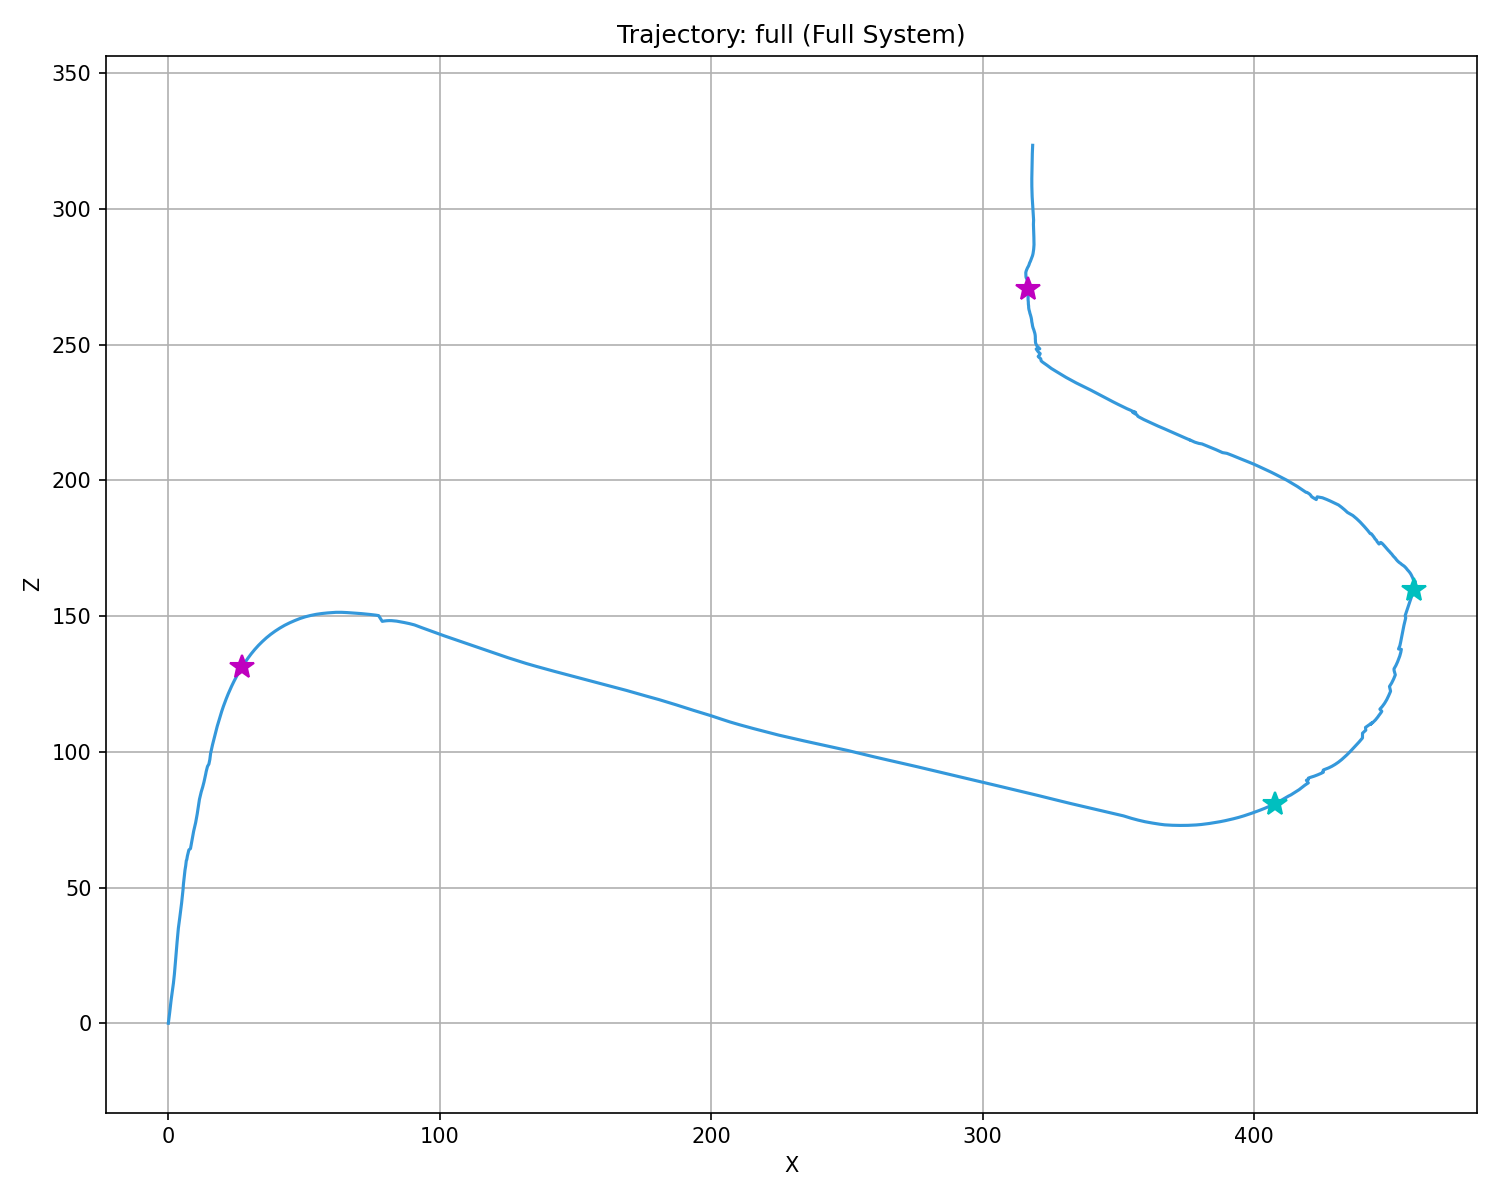
\includegraphics[width=0.75\linewidth]{driving_images/tracking_with_turn_dets.png}
    \caption{Turn detections from full VO pipeline. Purple and Blue stars show Right and Left turns respectively.}
    \label{fig:turn_detections}
\end{figure}

\subsection{Face Analysis (FR1.4)}
Facial landmark extraction was implemented using the InsightFace \cite{deng2019arcface} library, which was selected due to its robustness under varying lighting conditions and large face rotations. Google’s MediaPipe \cite{lugaresi2019mediapipe} was also tested, however it frequently failed to maintain landmark tracking when the face rotated too far, making it unsuitable for this application. Using the landmarks extracted by InsightFace, head pose angles were calculated using the PnP algorithm.\\

To classify discrete gaze directions, a sample video clip containing all required face directions was analysed (Figure \ref{fig:yawpitchroll_1}a). The yaw angle provided the most useful information for determining gaze direction, while pitch was found to be correlated with yaw due to the camera perspective. The estimated direction is visualised in Figure \ref{fig:gaze_examples} with a line coming from the nose.\\


\begin{figure}[H]
    \centering
    \subfigure[]{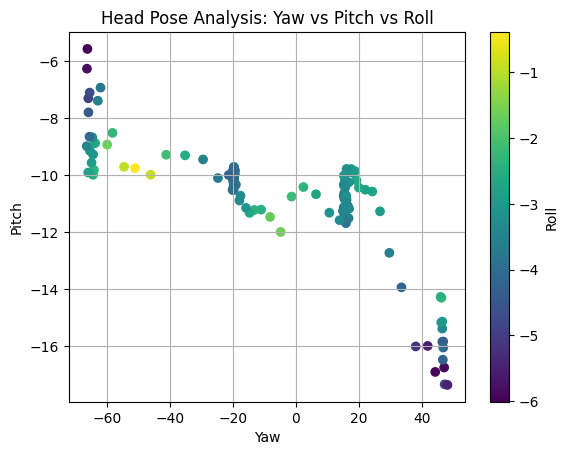
\includegraphics[width=0.49\textwidth]{face_analysis_images/head_angles_graph.png}}
    \subfigure[]{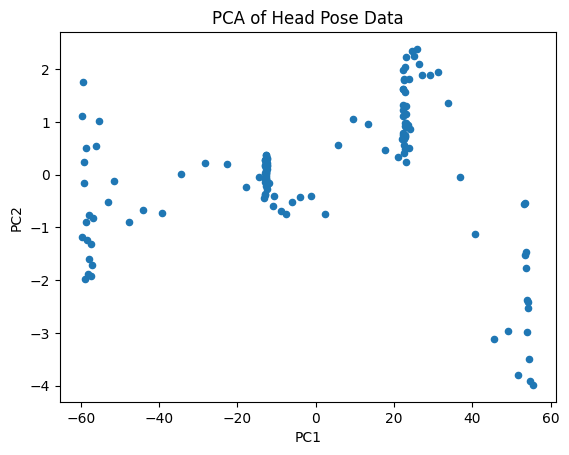
\includegraphics[width=0.49\textwidth]{face_analysis_images/pca_yaw_pitch_roll.png}} 
    \caption{(a) Yaw, Pitch, Roll from example video clip. (b) PCA transformation from 3D to 2D.}
    \label{fig:yawpitchroll_1}
\end{figure}

\begin{figure}[H]
    \centering
    \subfigure[]{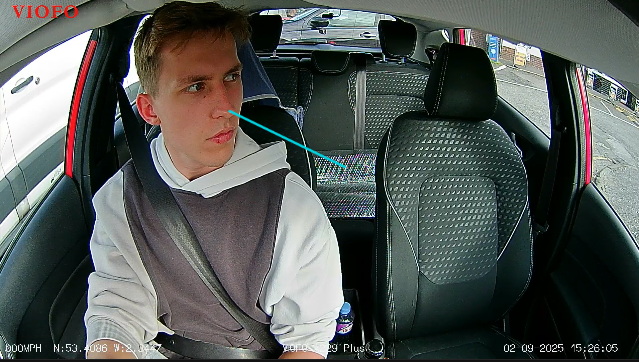
\includegraphics[width=0.32\textwidth]{driving_images/left_mirror.png}}
    \subfigure[]{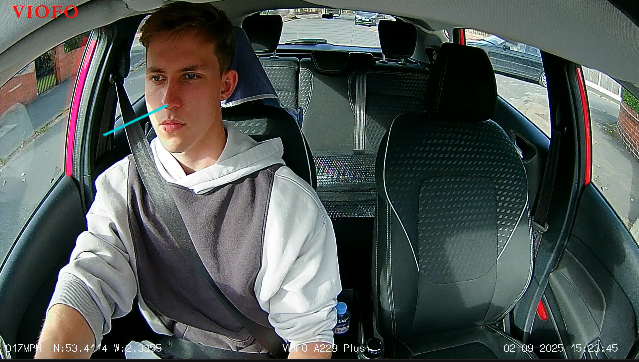
\includegraphics[width=0.32\textwidth]{driving_images/looking_forward.png}} 
    \subfigure[]{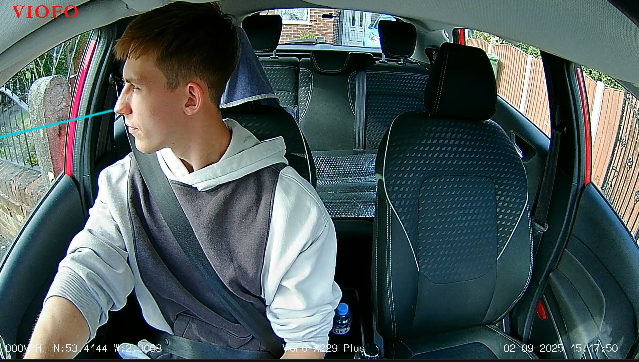
\includegraphics[width=0.32\textwidth]{driving_images/right_mirror.png}} 
    \caption{Angle estimations visualised: (a) Left mirror. (b) Looking ahead. (c) Right mirror.}
    \label{fig:gaze_examples}
\end{figure}

The raw angle data has three dimensions (yaw, pitch, roll), but not all contribute equally to distinguishing gaze directions. PCA was applied to project the data onto its two principal components (Figure \ref{fig:yawpitchroll_1}b), removing the least informative axis and producing tighter, more separable clusters for each gaze direction. The resulting two-dimensional representation also makes the classification boundaries easier to visualise and interpret during calibration. Initial experiments using K-Means clustering showed poor performance for outlying and ambiguous points, with several samples from the looking ahead and left mirror classes incorrectly grouped as rear mirror (Figure \ref{fig:yawpitchroll_2}a). In practice, the region corresponding to rear mirror checks occupies a much narrower area of the feature space than the other classes. For this reason, the data was manually labelled and an SVM classifier was trained instead, resulting in significantly more reliable classification (Figure \ref{fig:yawpitchroll_2}b).

\begin{figure}[H]
    \centering
    \subfigure[]{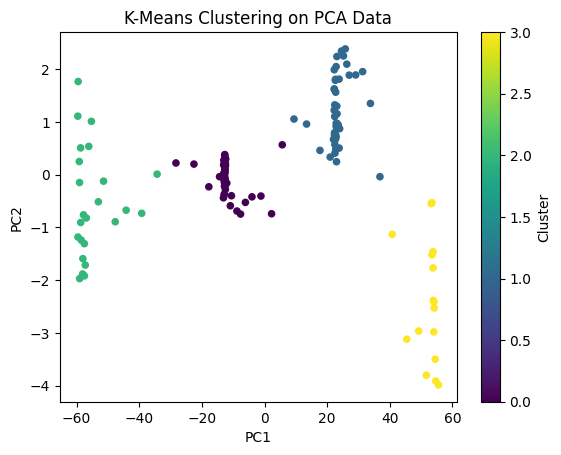
\includegraphics[width=0.49\textwidth]{face_analysis_images/kmeans_clusters.png}} 
    \subfigure[]{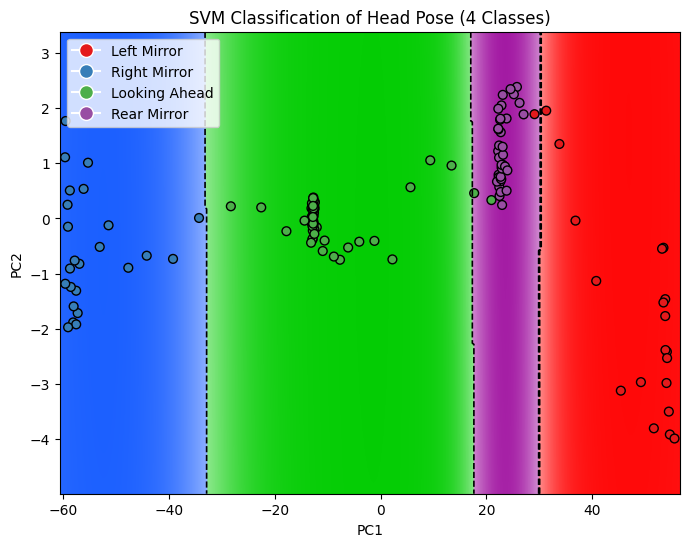
\includegraphics[width=0.49\textwidth]{face_analysis_images/svm_classification.png}} 
    \caption{(a) KMeans clustering results. (b) SVM classification results.}
    \label{fig:yawpitchroll_2}
\end{figure}

The gaze classifier was then integrated into the existing system. For each frame, facial landmarks and head pose angles are extracted, transformed using the PCA model, and classified into a gaze direction using the trained SVM. These observations are stored in the Safety Monitor buffer for use during mistake identification.

\subsection{Mistake Identification (FR1.5)}
The system identifies the driving mistake of failing to check mirrors prior to manoeuvres, including both lane changes and turns. When a manoeuvre is detected (either a lane crossing from the lane tracker or a turn event from the visual odometry module), the Safety Monitor queries the driver's gaze history over the preceding 5 seconds. If the driver checked the corresponding mirror (left mirror for rightward manoeuvres, right mirror for leftward manoeuvres) within this window, the event is classified as safe; otherwise, it is classified as unsafe. A rear mirror check is also noted if present, but is not sufficient on its own.\\

This rule-based heuristic was chosen over a learned classifier because the relationship between mirror checks and manoeuvres is well-defined by driving standards, making a simple threshold both interpretable and auditable. The UK Highway Code states that drivers should check mirrors ``in good time'' before any change of direction or speed \cite{highwaycode2025}, but does not prescribe a precise threshold. A 5-second lookback window was chosen as a practical compromise: long enough to capture a check performed shortly before the manoeuvre begins, but short enough that the observed traffic state remains relevant (Figure \ref{fig:safe_lane_change}).

\begin{figure}[H]
    \centering
    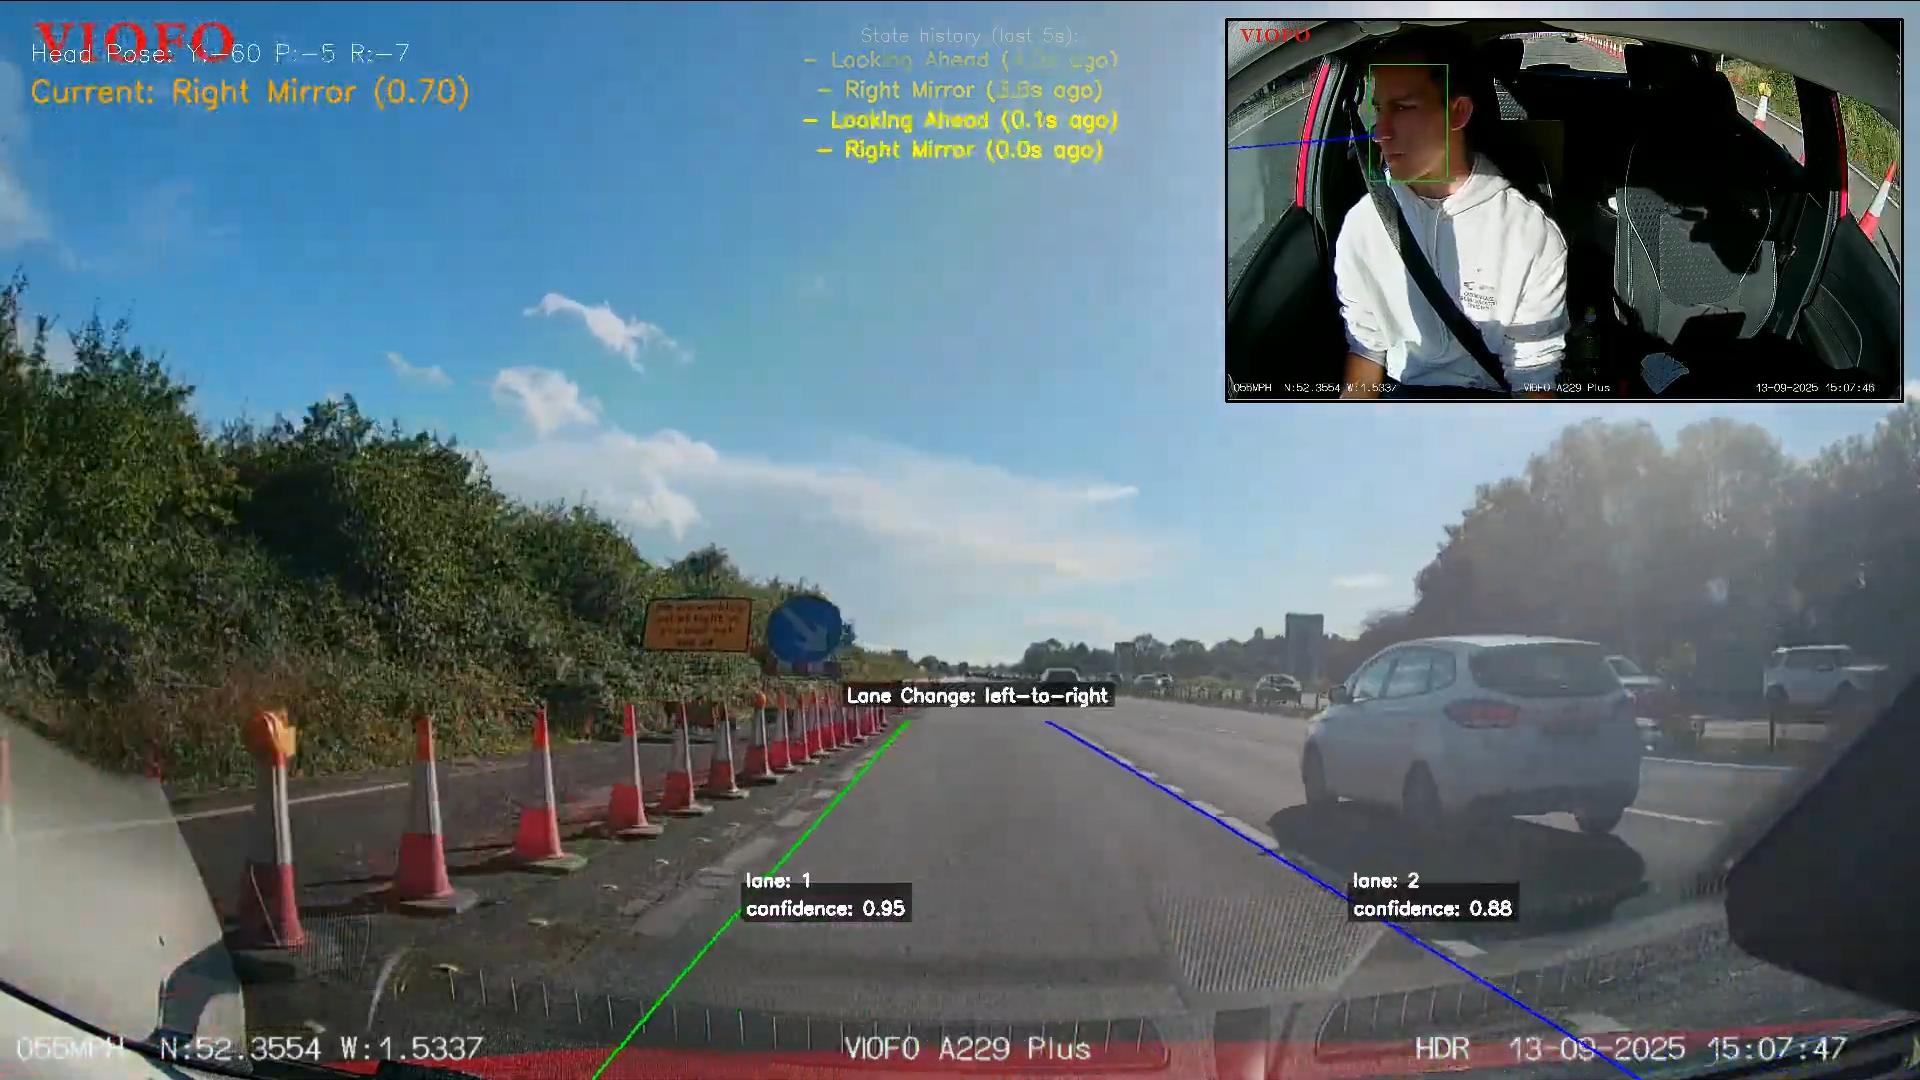
\includegraphics[width=0.8\linewidth]{driving_images/lanes+face.png}
    \caption{Safe lane change with log showing right mirror was checked 3 seconds before the merge.}
    \label{fig:safe_lane_change}
\end{figure}

\subsection{Web Application (FR2)}
% Seems a little implementation-heavy. Can you talk a bit more about the design?
The web application represents a substantial portion of the project's development effort. Beyond the core computer vision pipeline, building a responsive and functional system required solving a wide range of engineering challenges across the full stack: deploying a GPU-accelerated backend on shared university infrastructure, synchronising dual video streams with frame-level accuracy, and integrating a SLURM-based job queue transparently behind a web interface. A particular difficulty was designing workflows for tasks that are inherently user-specific and cannot be fully automated, such as gaze calibration, where each user's seating position and camera angle produce different head pose distributions that must be individually labelled and trained. Equally challenging was determining how to present the analysis results effectively; the interface needed to surface detected events, gaze history, timeline annotations and calibration tools without overwhelming users who are not technically trained. Iterative user testing was essential in finding the right balance between giving users enough control to calibrate and verify their results while keeping the interface intuitive. The resulting application allows users to upload their footage, which is analysed and the results presented on an interactive display with synchronised video playback and navigation to detected events.

\subsubsection{Overall System and Backend Design}
The application is designed as a Client-Server-Worker system to handle the heavy video processing requirements while keeping the UI smooth and responsive. A Python-based FastAPI server accepts requests from the React-based web app. The server offloads individual analysis work to sub-processes, which save the results on a centralised drive accessible by the server. These results can then be sent back to the web interface for viewing (Figure \ref{fig:architecture}).\\

\begin{figure}[H]
    \centering
    % TIKZ DIAGRAM START
    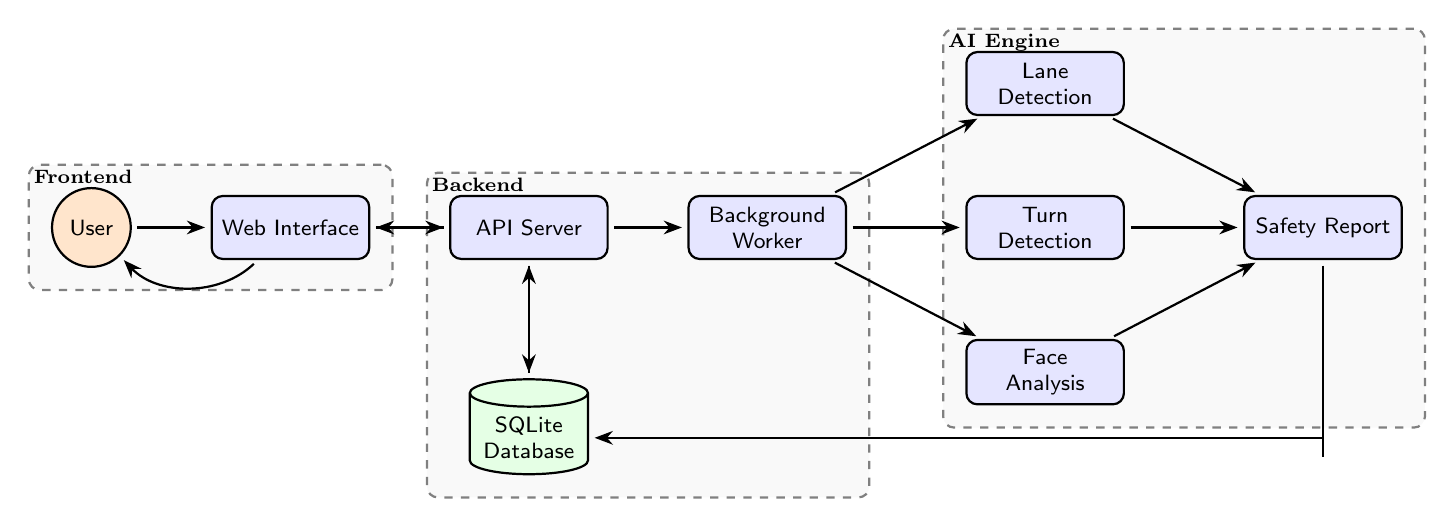
\begin{tikzpicture}[
        node distance=1.5cm and 1cm,
        font=\sffamily\footnotesize,
        % Define styles for the nodes
        process/.style={rectangle, draw=black, fill=blue!10, thick, minimum width=2cm, minimum height=0.8cm, rounded corners, align=center},
        user/.style={circle, draw=black, fill=orange!20, thick, minimum size=1cm, align=center},
        storage/.style={cylinder, shape border rotate=90, draw=black, fill=green!10, thick, aspect=0.25, minimum width=1.5cm, minimum height=1.2cm, align=center},
        group/.style={rectangle, draw=gray, thick, dashed, inner sep=8pt, rounded corners, fill=gray!5},
        myarrow/.style={->, >=Stealth, thick, shorten >=2pt, shorten <=2pt},
        label text/.style={midway, fill=white, font=\scriptsize\itshape, text=black, inner sep=1pt}
    ]

        % --- Nodes ---
        \node[user] (user) {User};
        \node[process, right=of user] (ui) {Web Interface};

        \node[process, right=of ui] (api) {API Server};
        \node[storage, below=of api] (db) {SQLite\\Database};
        \node[process, right=of api] (worker) {Background\\Worker};

        % AI task nodes stacked vertically
        \node[process, above right=1cm and 1.5cm of worker] (lanes) {Lane\\Detection};
        \node[process, right=1.5cm of worker] (vo) {Turn\\Detection};
        \node[process, below right=1cm and 1.5cm of worker] (face) {Face\\Analysis};
        \node[process, right=1.5cm of vo] (report) {Safety Report};

        % --- Groups ---
        \begin{scope}[on background layer]
            \node[group, fit=(user) (ui), label={[anchor=north west, inner sep=2pt, font=\scriptsize\bfseries]north west:Frontend}] (frontend) {};
            \node[group, fit=(api) (worker) (db), label={[anchor=north west, inner sep=2pt, font=\scriptsize\bfseries]north west:Backend}] (backend) {};
            \node[group, fit=(lanes) (face) (vo) (report), label={[anchor=north west, inner sep=2pt, font=\scriptsize\bfseries]north west:AI Engine}] (ai) {};
        \end{scope}

        % --- Edges ---
        \draw[myarrow] (user) -- (ui);
        \draw[myarrow] (ui) to[bend left=45] (user);

        \draw[myarrow] (ui) -- (api);
        \draw[myarrow] (api) -- (ui);
        \draw[myarrow] (api) -- (worker);
        \draw[myarrow] (api) -- (db);
        \draw[myarrow] (db) -- (api);

        % 1. Worker to AI tasks
        \draw[myarrow] (worker) -- (lanes);
        \draw[myarrow] (worker) -- (vo);
        \draw[myarrow] (worker) -- (face);

        % 2. AI tasks to Report
        \draw[myarrow] (lanes) -- (report);
        \draw[myarrow] (vo) -- (report);
        \draw[myarrow] (face) -- (report);

        \draw[myarrow] (report.south) -- ++(0,-2.5cm) |- (db.east);

    \end{tikzpicture}
    % TIKZ DIAGRAM END
    \caption{System Architecture Diagram showing the data flow between Frontend, Backend, and AI Workers.}
    \label{fig:architecture}
\end{figure}

When the server receives a request for an analysis job, it creates a new job object in a SQLite database. This job entry can be queried by the front-end to determine the current progress of the analysis or whether any errors have occurred. The server then spawns a new Python process to complete the analysis task. By using separate processes rather than threads, the system avoids memory management-based limitations imposed by Python’s Global Interpreter Lock, allowing multiple analysis jobs to run in parallel. This design allows multiple jobs to be queued and processed without overloading the server, ensuring that the application remains responsive.\\

A one-process-per-request strategy was chosen over maintaining a pool of idle processes, as the overhead of process creation is insignificant compared to the duration of the analysis tasks. This approach avoids unnecessary resource usage while maintaining flexibility and scalability as the system workload changes.\\

The system was initially developed and tested locally, with both the frontend and backend running on the development machine. However, conducting a user study required the application to be accessible remotely so that participants could upload their own footage. To achieve this, the application was deployed to the university’s DCS shared server infrastructure. The FastAPI backend and React frontend were served over HTTPS using self-signed SSL certificates, with the backend bound to a dedicated port and the frontend built and served via Vite’s preview mode. Video files and analysis outputs were stored on the DCS large shared filesystem, which is accessible to both the server process and any SLURM cluster jobs. A startup script was written to launch both services, configure the correct paths, and activate the required Python virtual environment and Conda environment for GPU dependencies.\\

SLURM cluster integration was added via SSH tunnelling, allowing analysis and recalibration jobs to be submitted to the university’s GPU cluster. Offloading to the cluster significantly reduces processing time compared to running on the shared server’s CPU, as the Mask R-CNN inference and face analysis models benefit substantially from GPU acceleration. However, the SLURM scheduling system introduces a trade-off: during periods of high cluster utilisation, jobs may be queued behind other users’ workloads, meaning analysis start times are unpredictable. To manage this, the backend polls SLURM job status and relays queue position and estimated wait times to the frontend, so users are kept informed rather than left waiting without feedback. The backend manages job submission, monitors SLURM job status, and retrieves results from the shared filesystem, abstracting the cluster interaction entirely from the user.\\

\subsubsection{User Authentication and Account System}
The initial prototype operated without user accounts, meaning anyone with the URL could upload videos and view all results. This was acceptable during development but inadequate for real-world use, where analysis results contain sensitive footage and users need to manage their own history. A user account system was therefore added, with registration, login, and per-user access control over uploaded videos and results.\\

Authentication is handled via JSON Web Tokens (JWT) with a 7-day expiry limit. This was chosen over session-based authentication because the stateless nature of JWTs avoids the need for server-side session storage and simplifies the deployment for the backend. Tokens are generated by the FastAPI backend and verified on each protected request. Additionally, account activation requires admin approval after registration. This effectively works as a whitelist, which allows the researcher to carefully authenticate each account, preventing unauthorised access. It also means the admin can check each user’s driver’s license as per the requirements by the ethical approval board.

\subsubsection{Upload Flow and Video Synchronisation}
The frontend was built using React with Vite as the build tool, and Bootstrap for layout and styling. React was chosen for its component-based architecture, which suited the modular nature of the interface: the video player, timeline, calibration editor and upload flow are all independent components that share state through React’s context system. Vite was preferred over Create React App due to its significantly faster development server and hot module replacement, which shortened the iteration cycle during UI development. Axios handles HTTP communication with the FastAPI backend.\\

The upload flow supports the submission of multiple consecutive video files, which is necessary as dash-cam systems use loop-recording rather than saving entire driving sessions in a single file. Files are uploaded in segments and spliced server-side using FFmpeg’s concat demuxer, handling the common case of multiple sequential recordings transparently.\\

\begin{figure}[H]
    \centering
    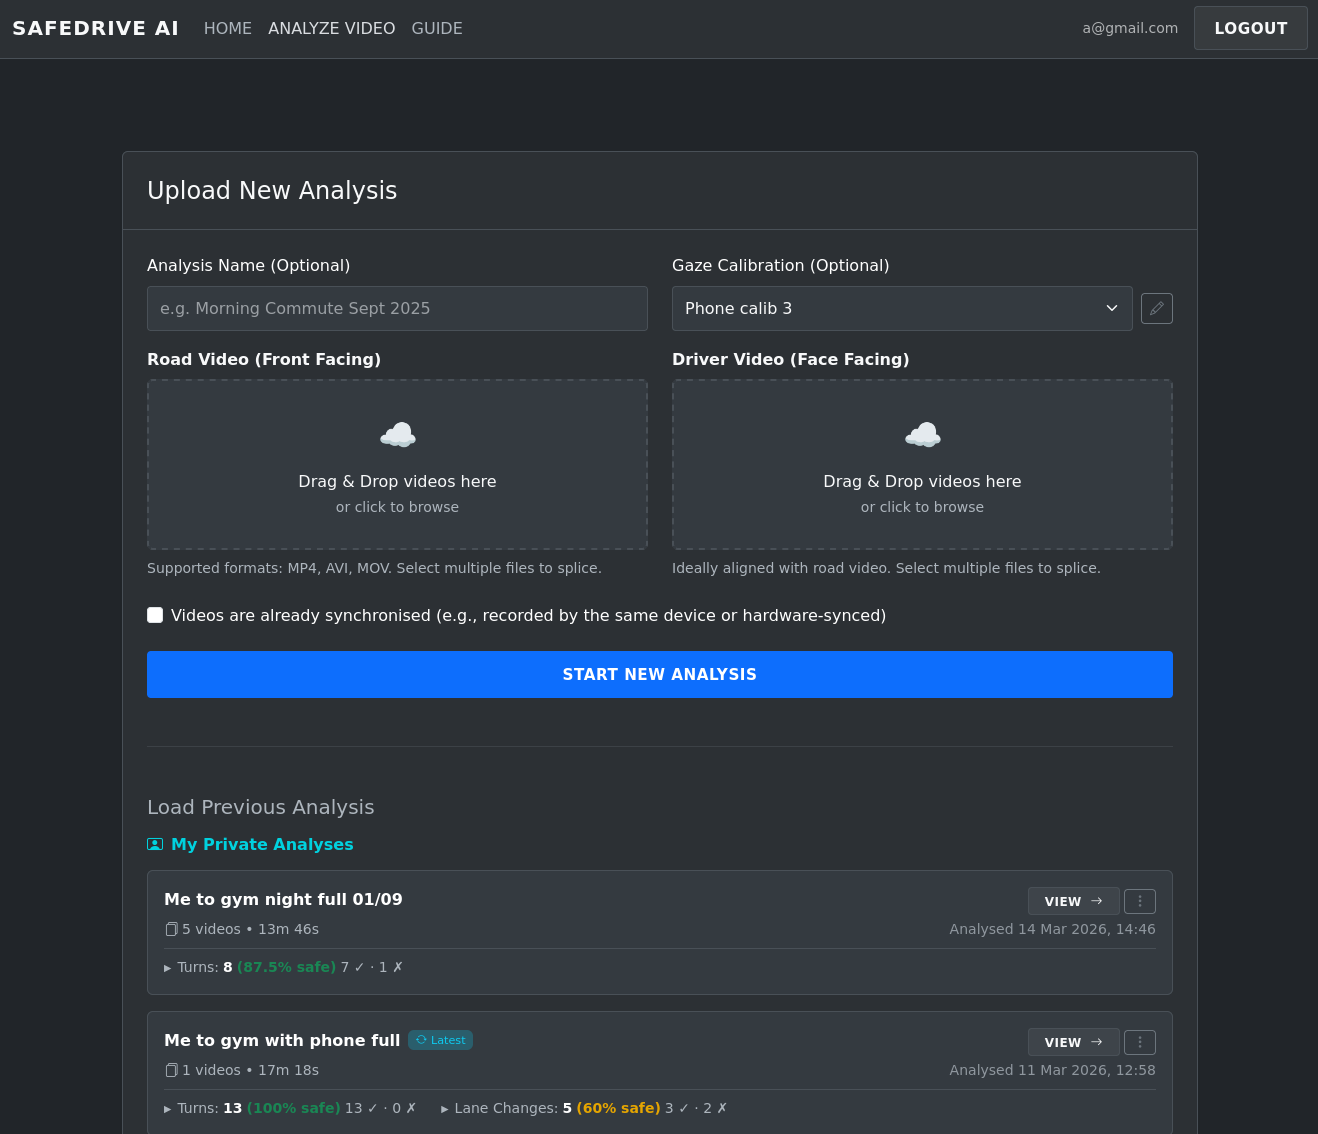
\includegraphics[width=0.8\linewidth]{website_images/analysis_submission.png}
    \caption{Screenshot of the video submission page.}
    \label{fig:video_submission}
\end{figure}

A key usability challenge was that users cannot be expected to manually align their two video streams before uploading. Most users record with separate devices (e.g.\ a dedicated dash-cam and a phone mounted on the dashboard), which start at different times and have no shared clock signal. Requiring users to determine the offset themselves using external video editing tools would make the application impractical for the target audience of learner drivers and their supervisors. The system therefore needed an automated synchronisation step that handles alignment transparently, while still giving users the ability to verify and correct the result when the automatic method is uncertain.\\

The synchronisation algorithm exploits the fact that both cameras share the same acoustic environment inside the vehicle. Engine noise, speech, indicator clicks and road noise are captured by both microphones, providing a natural reference signal for alignment. The process begins by extracting mono PCM audio from both videos using FFmpeg, downsampled to 4000\,Hz and capped at the first 120 seconds, which is sufficient for detecting the offset while keeping computation fast. The extracted signals are normalised by subtracting the mean and dividing by the standard deviation, removing differences in microphone sensitivity and recording volume.\\

The temporal offset is then computed using FFT-based cross-correlation via SciPy’s \texttt{fftconvolve} function. Cross-correlation measures the similarity between two signals as a function of a time lag applied to one of them. By computing this in the frequency domain using the Fast Fourier Transform, the operation runs efficiently even on long audio signals. The lag corresponding to the peak of the cross-correlation function gives the sample offset between the two recordings, which is converted to seconds using the known sample rate. A confidence score is derived by normalising the peak correlation value relative to the total signal energy, producing a value between 0 and 1 that indicates how reliable the computed offset is.\\

Once the offset is determined, both videos are trimmed to their overlapping temporal window. If the offset is positive (the cabin video starts after the road video), the road video is trimmed from the front by the offset duration; if negative, the cabin video is trimmed instead. A minimum overlap of 2 seconds is enforced to ensure there is sufficient synchronised content for analysis.\\

The synchronisation result is presented to the user through a confirmation interface before analysis begins (Figure \ref{fig:audio_sync}). The interface displays both audio waveforms on an interactive canvas, with a visual indicator showing the computed alignment point. A confidence badge (high, medium or low) communicates the reliability of the automatic result. If confidence is low, which can occur when the two cameras are in very different acoustic environments or one has no audio track, the user is warned and can manually adjust the offset using fine-grained controls ($\pm$0.1\,s and $\pm$0.01\,s increments) or by dragging the waveforms directly. A synchronised preview playback allows the user to verify the alignment visually before confirming. Once confirmed, the synchronised videos are submitted for analysis and the user is shown progress updates until processing completes.\\

\begin{figure}[H]
    \centering
    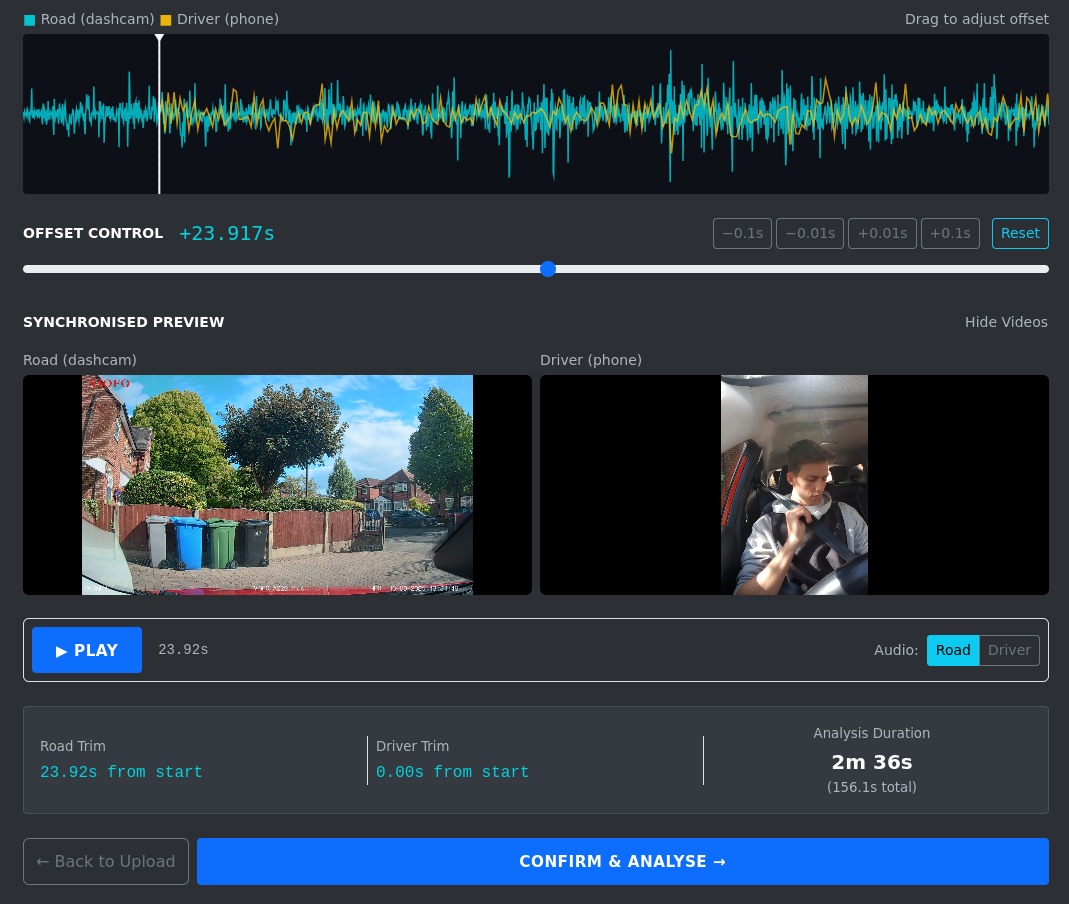
\includegraphics[width=0.8\linewidth]{website_images/audio_sync_screen.png}
    \caption{Synchronisation confirmation interface showing dual waveforms and manual adjustment controls.}
    \label{fig:audio_sync}
\end{figure}

\subsubsection{Results Display}
After analysis is complete, the application presents the detected results to the user, including safe and unsafe manoeuvre events (lane changes and turns). A central design challenge was presenting the output of three separate analysis modules (lane detection, turn detection, gaze classification) in a unified view that users could interpret without technical knowledge. The solution was a custom timeline bar that encodes detected events and driver gaze information as colour-coded segments along the video’s duration, enabling the user to see the relationship between manoeuvres and mirror checks at a glance rather than splitting attention between different interface elements. Clicking on an event in the timeline seeks both video streams to that timestamp, keeping them synchronised via a drift correction mechanism that monitors the two video elements and resyncs them if they diverge by more than 0.3 seconds, compensating for browser-level timing inconsistencies. Additional logs of detected events and gaze transitions are displayed alongside the videos, making the system’s reasoning transparent and allowing users to understand why a particular event was classified as safe or unsafe.\\

\begin{figure}[H]
    \centering
    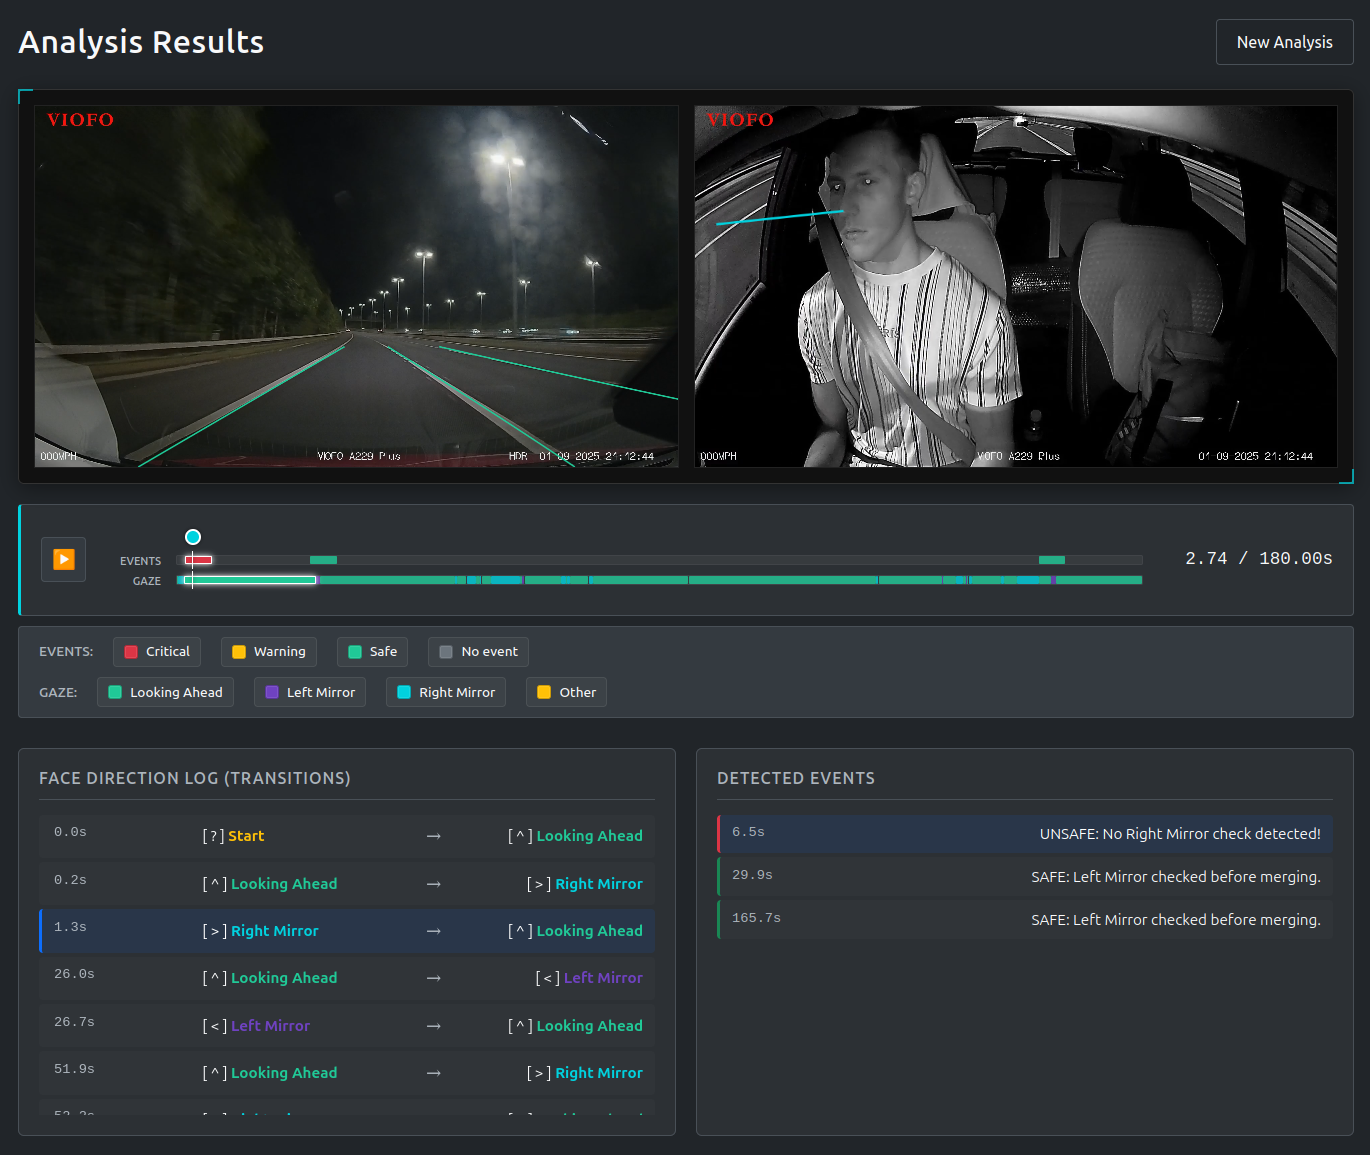
\includegraphics[width=1\linewidth]{website_images/web_display_1.png}
    \caption{Web application results page with synchronised dual-video playback, custom event timeline and event logs.}
    \label{fig:web_app_design}
\end{figure}

\subsubsection{Per-User Gaze Calibration}
The default SVM gaze classifier was trained on head pose data collected from a single individual in a specific vehicle with a specific camera position. During user testing, it became clear that this model did not generalise well: differences in seating position, camera angle, head size and facial geometry meant that the decision boundaries trained on one person’s data frequently misclassified another’s gaze directions. For example, one tester’s ``looking ahead’’ yaw angle fell within the region the default model classified as ``left mirror’’, because their camera was mounted at a different angle. Since the gaze classifier is the foundation of all safety judgements, poor classification accuracy renders the entire system unreliable. This motivated the development of a per-user calibration system as an extension.\\

The initial calibration interface provided a clip editor (Figure \ref{fig:calib_editors}a), where users mark time segments in their previously analysed videos and label them with the corresponding gaze direction (e.g.\ ``Left Mirror’’, ``Looking Ahead’’). The system extracts the stored head pose angles (yaw, pitch, roll) from the existing analysis results for the marked segments, avoiding the need to re-run face detection. Once sufficient samples are collected (a minimum of 3 per mandatory class: Left Mirror, Right Mirror, Looking Ahead; with Rear Mirror optional since not all vehicles have a visible interior rear-view mirror), the user triggers model training, which fits a new PCA transformer and SVM classifier on their personal data. Diagnostic plots (head pose scatter, PCA projection, and SVM decision boundary) are generated and displayed so the user can visually verify that the class regions correspond to their actual gaze directions before using the model.\\

A key design challenge was enabling re-analysis with a new calibration without re-running the full video pipeline, which takes several minutes per video and requires GPU resources. Since the head pose angles (yaw, pitch, roll) are already stored per-frame in the analysis results, a lightweight \texttt{recalibrate\_headless} script was developed that loads the user’s PCA and SVM models, batch-classifies all stored frames, and replays the safety monitor logic against the updated gaze labels. This completes in seconds on CPU alone, making it practical for users to iterate on their calibration, adjusting training samples and immediately seeing how the changes affect their safety results.\\

During early user testing, several participants found the clip editor daunting, as it required them to scrub through their videos to find segments where they were looking at each mirror and then mark precise time boundaries. This process typically took around five minutes of trial and error before users felt confident in their calibration. To address this, a point editor (Figure \ref{fig:calib_editors}b) was added, allowing users to directly view, add, or remove individual training points on the PCA scatter plot rather than working through video clips. This reduced the calibration process to under a minute for most users, since they could simply correct the few misclassified points rather than re-selecting entire video segments. Some users still found the clip editor useful when they had deliberately looked at each mirror at the start of a recording for the purpose of calibration, so both interfaces were retained. The interface also supports ``Save As’’ (duplicating a calibration to experiment with different training sets without losing the original) and renaming.

\begin{figure}[H]
    \centering
    \subfigure[]{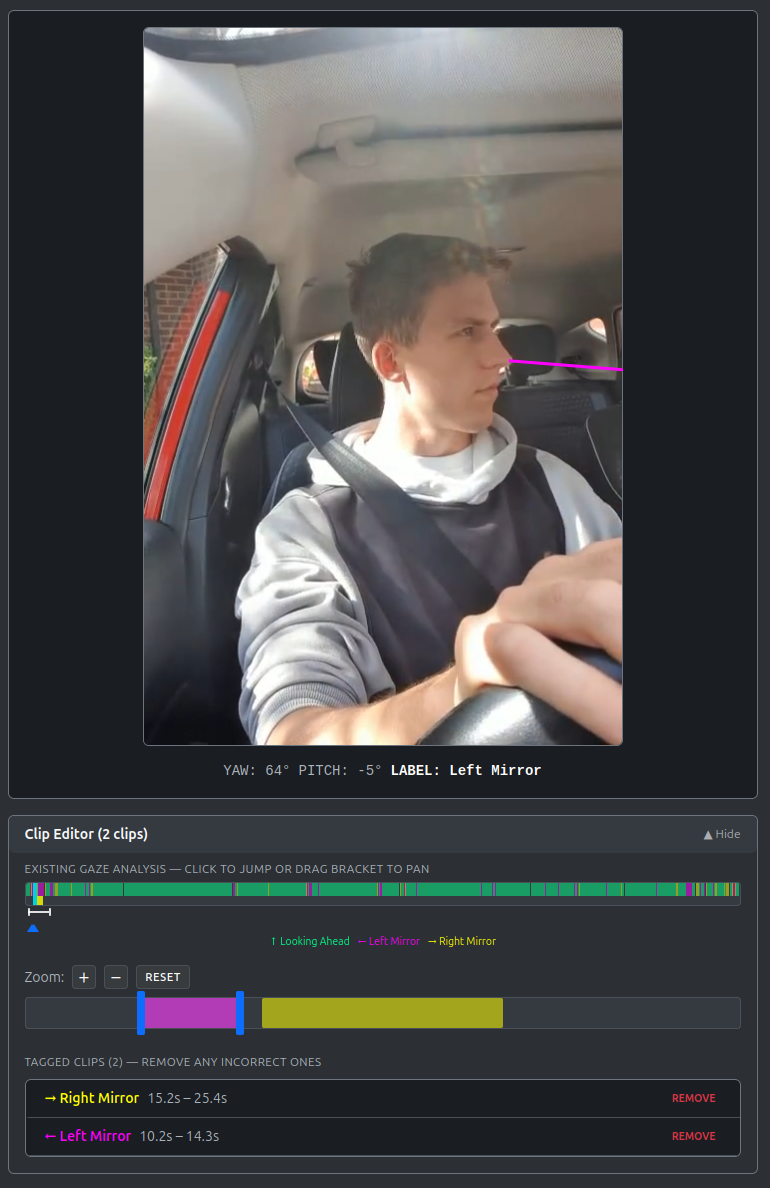
\includegraphics[width=0.49\textwidth]{website_images/clip_editor.png}}
    \subfigure[]{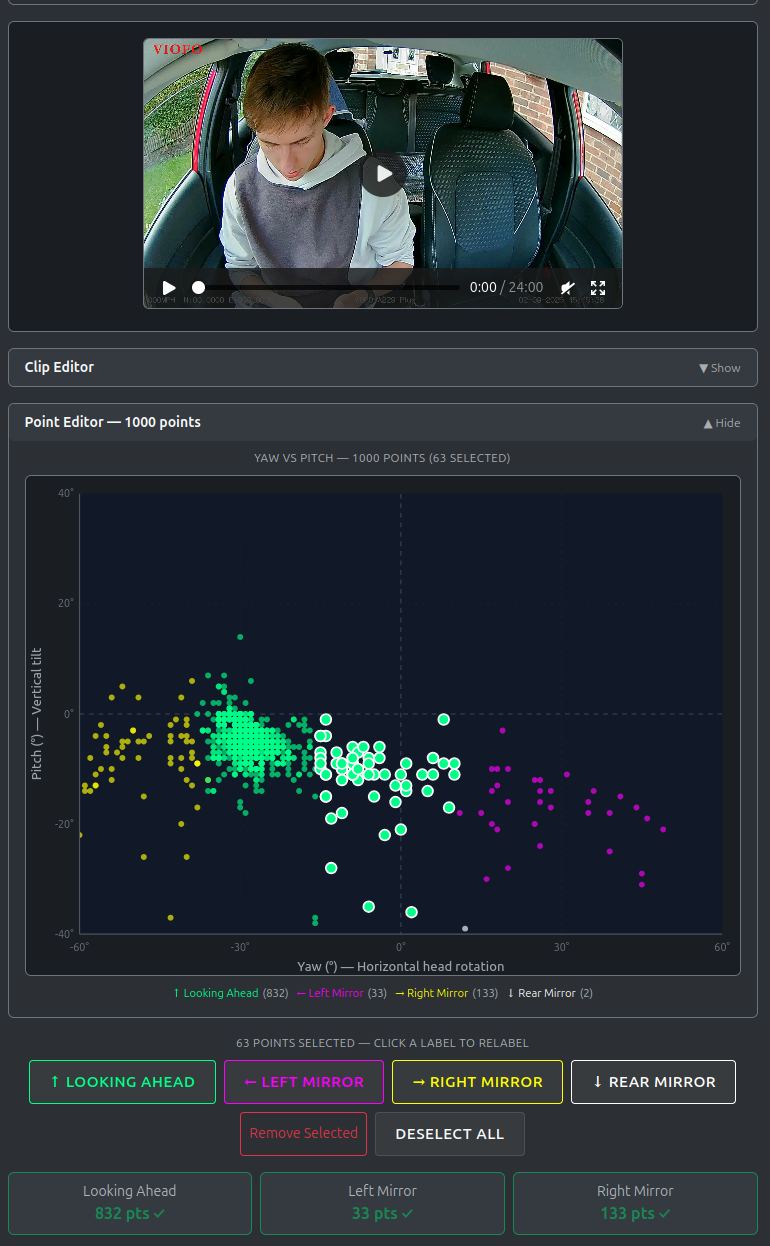
\includegraphics[width=0.49\textwidth]{website_images/point_editor.png}}
    \caption{(a) Clip editor for selecting labelled video segments. (b) Point editor for directly modifying training samples on the PCA scatter plot.}
    \label{fig:calib_editors}
\end{figure}

Calibration is optional; users who skip it are evaluated against the default model, which may produce unreliable results depending on their camera position and seating arrangement. Ideally, calibration would be embedded into a dedicated mobile recording application that guides the user through a short setup sequence at the start of each recording, using audio cues to prompt them to look at each mirror in turn. Such an application would also eliminate the current requirement for users to install a third-party app for face recording, since mobile operating systems do not permit background video capture from the built-in camera app. Developing a mobile-native solution would therefore simplify both the recording and calibration workflows, and is a clear avenue for future development.

\subsubsection{Privacy and Video Output Processing}
The driver-facing camera inevitably captures passengers and, depending on the camera’s field of view, potentially pedestrians or other bystanders visible through windows. Distributing or displaying this footage without consent raises ethical and legal concerns, particularly under GDPR. Since the system’s analysis only requires the driver’s face, all other faces can be obscured without any loss of functionality.\\

During analysis, the \texttt{FaceAnalyzer} identifies the driver using a heuristic: in landscape-oriented footage (the typical dash-cam configuration), the driver is the largest face on the left side of the frame (corresponding to the right-hand-drive UK vehicles used in testing). In portrait orientation, as may occur with a phone-based camera, the largest face overall is selected, as spatial position is less reliable. All other detected faces are blurred using a Gaussian kernel sized proportionally to the face bounding box, ensuring sufficient obscuration regardless of distance from the camera. The blurred frames are written as the output video, so the original unblurred footage is never stored on the server. Gaussian blurring was chosen over pixelation because it is less visually jarring while still being irreversible, and over full-frame blurring because retaining the driver’s face allows manual verification of gaze classifications during evaluation.\\

% TODO: Insert images of blurred face examples
During user testing on mobile devices, it was observed that loading the full-resolution output videos (1080p) over the university’s Wi-Fi caused significant buffering, particularly when both road and driver-facing streams needed to be loaded simultaneously. Since two concurrent video streams double the bandwidth requirement compared to a single-video application, adaptive quality selection was particularly important. To address this, the system generates multiple quality variants (720p and 480p) of both output videos after analysis completes, using FFmpeg, a widely-used open-source multimedia framework, to transcode into web-compatible H.264. Upscaling is avoided: variants are only generated when the source resolution exceeds the target. The frontend estimates the user’s effective bandwidth and automatically selects an appropriate resolution, with the option to manually override.

\subsubsection{Evaluation Infrastructure}
Evaluating the accuracy of the system’s safety judgements requires ground truth, which is difficult to obtain at scale. Rather than relying solely on the author’s own labelling, a user error reporting mechanism was integrated into the results page. When viewing an analysis, users can flag events they believe are incorrect (either false positives where events are flagged as unsafe that were actually safe, or false negatives where unsafe events were missed), with the report automatically capturing the current video timestamp for context. These reports are stored in the database and presented to the author, providing a source of labelled feedback for current accuracy measurement and evaluation, and to inform future improvements to detection thresholds and classification models.\\


As the system was deployed for user testing with multiple participants, it became necessary to monitor usage, review reported errors, and manage jobs centrally. An administrator dashboard was developed, restricted to users with an admin role (enforced via a claim in the JWT token). In practice, the author is the only administrator, and the dashboard served as a central tool for ongoing research and system improvement.\\

The dashboard provides per-user safety event analytics, displaying aggregated counts of safe and unsafe events across all of a user’s analyses to identify patterns in system performance across different drivers and camera setups. Job management capabilities allow administrators to reassign analyses between users and monitor batch SLURM-submitted jobs. User-submitted error reports (false positives and false negatives) are displayed inline alongside the corresponding analysis results and synchronised video playback, allowing the author to verify reports without switching between separate views. Administrators can also download 15-second video clips centred around specific events, which proved useful for quickly reviewing flagged errors without loading full recordings.\\

This infrastructure proved valuable beyond simple monitoring. By reviewing user-reported false positives and false negatives, the author was able to measure the system’s detection accuracy across a range of real driving scenarios. The dashboard also enabled the discovery of specific failure modes; for example, reviewing reported errors in turn detection led to the identification and correction of the global angle accumulation issue discussed in Section 3.3. Without centralised access to user reports and the ability to replay events in context, such improvements would have been significantly harder to diagnose.

% TODO: Insert screenshot of admin dashboard

\subsubsection{Error Handling}
Error handling was hardened across the upload, synchronisation and analysis pipeline to gracefully handle oversized files, network interruptions, malformed video codecs and out-of-memory conditions on the GPU. A ``Getting Started’’ guide page was added to the frontend to help new users understand the required dual-camera setup and upload process, reducing support requests during the evaluation phase.

% Consider showing the "Getting Started" guide.

\newpage

\section{Evaluation Methodology}
% I can see this is a plan rather than a draft. It looks good. I know we've discussed this before, but if you can compare against existing work in any way, that would be good. Did you do any testing?
Explain the process(es) that I have gone through in order to evaluate the project. Justify that they are objective (or as much as I can make them), and help prove the technical contribution of the project.\\

Possible results/evaluation inclusions in report:
\begin{itemize}
    \item Users have option to report mistakes in the application - can give \% of mistakes (FP/FN) compared to correct detections
    \item Manually label parts of my own dataset to get \% correct event detections, can compare different versions of the models/system with this to show higher detection counts as we add/fine-tune features and do more research
    \item Difficult to judge gaze classifications since this is user-specific (and needs to be user-calibrated), however would be interesting to investigate how many points you need to get a sufficient accuracy, by labelling some gaze clip myself (for validation) and then using an SVM trained on 10 frames, 100 frames, 1000 frames etc. to show how much calibration the user needs to do for example?
    \item Ask passenger to identify how many errors they spotted, and compare this to the system
    \item Qualitative evaluation of the application by users:
    \begin{itemize}
        \item `Would you use this/recommend this to someone learning?'
        \item `Do you think this is a useful tool?'
    \end{itemize}
\end{itemize}

\newpage

\section{Results}
Show the results - graphs, diagrams, tables of the evaluation techniques from the previous section.

\newpage

\section{Conclusion and Future Work}
Discuss how this project can be extended further, what other use-cases there are for the technology. Plan to include: 
\begin{itemize}
    \item How the current features could be improved
    \item More features for detecting mistakes (how these could be implemented - would they be simple? Which to prioritise first?)
    \item Other use-cases: not just for learner drivers: could be used for insurance systems or training ADAS systems by auto-labelling clips of manouevres for example.
\end{itemize}

\newpage

\section{Self-Assessment}
Covers the author's own assessment of the success of the project, in terms of technical contribution, usefulness, limitations.\\

Overall, the project was a success - it shows that a computer vision system can indeed identify driving errors which are difficult for non-trained passengers to spot. While the models do not perform with 100\% accuracy, as limited by the constraints (time, cost, resources, scope) of the project, the project overall does show that such a system would be helpful to people, and with a larger budget, scope, industry connections etc. this could be a successful business idea. It can also be applied to other industries such as insurance and in-car safety mechanisms. Since there don't currently exist systems that match what the project does, it provides justification for further developing the application or similar applications, and it presents a benchmark for future researchers to compare against. 

\section{Acknowledgements}
Thank yous to supervisor, external advisor, DCS tech, other stakeholders...

\bibliography{progress_report_bibliography}

%========== Project specification left as appendix to document ==========%


\end{document}
